%%%%%%%%%%%%%%%%%%%%%%%%%%%%%%%%%%%%%%%%%%%%%%%%%%%%%%%%%%%%%%%%%%%%%%%%%%%%%%%%%%%%%%%%%%%%%%%%
% UNIVOTE LATEX TEMPLATE
%%%%%%%%%%%%%%%%%%%%%%%%%%%%%%%%%%%%%%%%%%%%%%%%%%%%%%%%%%%%%%%%%%%%%%%%%%%%%%%%%%%%%%%%%%%%%%%%

\documentclass[bibtotoc,halfparskip,oneside]{scrreprt}

\usepackage{import}
\import{../latex/}{english.tex} 
% you must set the path according to the current document folder
% use "german.tex" for documents in german and "english.tex" for documents in english
\inputpath{{listings/}{figures/}}

\usepackage{enumitem}
%\usepackage[enable]{easy-todo}
\usepackage{cleveref}
\usepackage{lscape}
\usepackage{multirow}
\usepackage{seqsplit}

\setcounter{secnumdepth}{4}
\renewcommand{\thesubsubsection}{\alph{subsubsection}}
\renewcommand*{\othersectionlevelsformat}[3]{% 
  #3% 
  \begingroup 
    \edef\istlevel{#1}\def\solllevel{subsubsection}% 
    \ifx\istlevel\solllevel )\else\autodot\fi 
  \endgroup 
  \enskip 
} 



%%%%%%%%%%%%%%%%%%%%%%%%%%%%%%%%%%%%%%%%%%%%%%%%%%%%%%%%%%%%%%%%%%%%%%%%%%%%%%%%%%%%%%%%%%%%%%%%
% Definition of Symbols
% Note: Every symbol defined here should be mentioned in the glossary
%%%%%%%%%%%%%%%%%%%%%%%%%%%%%%%%%%%%%%%%%%%%%%%%%%%%%%%%%%%%%%%%%%%%%%%%%%%%%%%%%%%%%%%%%%%%%%%%

\newcommand{\hex}[1]{\ensuremath{\mathtt{#1}}}
\newcommand{\HEX}[1]{\ensuremath{\mathtt{#1}_{16}}}
\newcommand{\bin}[1]{\ensuremath{\mathtt{#1}}}
\newcommand{\BIN}[1]{\ensuremath{\mathtt{#1}_{2}}}
\newcommand{\str}[1]{\ensuremath{\text{\texttt{"#1"}}}}
\newcommand{\chr}[1]{\ensuremath{\text{\texttt{'#1'}}}}
\newcommand{\conc}{\ensuremath{\;||\;}}



\newcommand{\eid}{\mathit{id}\xspace}
\newcommand{\descrElection}{\mathit{election}\xspace}
\newcommand{\descrOptions}{\mathit{options}\xspace}
\newcommand{\period}{\mathit{period}\xspace}
\newcommand{\security}{\mathit{securityLevel}\xspace}
\newcommand{\cred}[1]{cred_{#1}\xspace}

\newcommand{\sk}[1]{\mathit{sk}_{#1}\xspace}
\newcommand{\vk}[1]{\mathit{vk}_{#1}\xspace}
\newcommand{\vkprime}[1]{\mathit{vk}'_{#1}\xspace}
\newcommand{\vkbar}[1]{\bar{\mathit{vk}}_{#1}\xspace}
\newcommand{\vkbarprime}[1]{\bar{\mathit{vk}}'_{#1}\xspace}
\newcommand{\vkhat}[1]{\hat{\mathit{vk}}_{#1}\xspace}
\newcommand{\vkhatprime}[1]{\hat{\mathit{vk}}'_{#1}\xspace}

\newcommand{\SK}[1]{\sk{_#1}\xspace}
\newcommand{\VK}[1]{\vk{_#1}\xspace}

\newcommand{\CA}{\ensuremath{\mathsf{CA}}\xspace}
\newcommand{\Prover}{\ensuremath{\mathsf{P}}\xspace}
\newcommand{\Verifier}{\ensuremath{\mathsf{V}}\xspace}
\newcommand{\User}{\ensuremath{\mathsf{U}}\xspace}
\newcommand{\IdentityProvider}{\ensuremath{\mathsf{U}}\xspace}

\newcommand{\RA}{\ensuremath{\mathsf{RA}}\xspace}
\newcommand{\EA}{\ensuremath{\mathsf{EA}}\xspace}
\newcommand{\EC}{\ensuremath{\mathsf{EC}}\xspace}
\newcommand{\UBC}{\ensuremath{\mathsf{UBC}}\xspace}
\newcommand{\UBV}{\ensuremath{\mathsf{UBV}}\xspace}
\newcommand{\UC}{\ensuremath{\mathsf{UC}}\xspace}
\newcommand{\Tallier}[1]{\ensuremath{\mathsf{T}_{#1}}\xspace}
\newcommand{\Mixer}[1]{\ensuremath{\mathsf{M}_{#1}}\xspace}
\newcommand{\Voter}[1]{\ensuremath{\mathsf{V}_{#1}}\xspace}

%%%%%%%%%%%%%%%%%%%%%%%%%%%%%%%%%%%%%%%%%%%%%%%%%%%%%%%%%%%%%%%%%%%%%%%%%%%%%%%%%%%%%%%%%%%%%%%%
% Listing for JSON
%%%%%%%%%%%%%%%%%%%%%%%%%%%%%%%%%%%%%%%%%%%%%%%%%%%%%%%%%%%%%%%%%%%%%%%%%%%%%%%%%%%%%%%%%%%%%%%%

%\usepackage{bera}% optional: just to have a nice mono-spaced font
\usepackage{listings}
\usepackage{xcolor}

\colorlet{punct}{red!60!black}
\definecolor{background}{HTML}{EEEEEE}
\definecolor{delim}{RGB}{20,105,176}
\colorlet{numb}{magenta!60!black}

\lstdefinelanguage{json}{
    basicstyle=\normalfont\ttfamily,
    numbers=left,
    numberstyle=\scriptsize,
    stepnumber=1,
    numbersep=8pt,
    showstringspaces=false,
    breaklines=true,
    frame=lines,
    backgroundcolor=\color{background},
    literate=
     *{0}{{{\color{numb}0}}}{1}
      {1}{{{\color{numb}1}}}{1}
      {2}{{{\color{numb}2}}}{1}
      {3}{{{\color{numb}3}}}{1}
      {4}{{{\color{numb}4}}}{1}
      {5}{{{\color{numb}5}}}{1}
      {6}{{{\color{numb}6}}}{1}
      {7}{{{\color{numb}7}}}{1}
      {8}{{{\color{numb}8}}}{1}
      {9}{{{\color{numb}9}}}{1}
      {:}{{{\color{punct}{:}}}}{1}
      {,}{{{\color{punct}{,}}}}{1}
      {\{}{{{\color{delim}{\{}}}}{1}
      {\}}{{{\color{delim}{\}}}}}{1}
      {[}{{{\color{delim}{[}}}}{1}
      {]}{{{\color{delim}{]}}}}{1},
}

\begin{document}

\title{UniVote2 System Specification}
\maketitle

\begin{versionhistory}
	\vhEntry{0.1}{14.07.2012}{Rolf Haenni}{Initial Draft.}
	\vhEntry{0.2}{15.08.2012}{Rolf Haenni}{Complete revision of initial draft.}
	\vhEntry{0.3}{10.09.2012}{Rolf Haenni}{Includes now the case of late registrations.}
	\vhEntry{0.4}{13.03.2013}{Rolf Haenni}{Improved ballot acceptance and closing the urn.}
	\vhEntry{0.5}{04.04.2013}{Rolf Haenni}{Revised section on zero-knowledge proofs.}
	\vhEntry{0.5.1}{30.04.2013}{Rolf Haenni}{Improved notational consistency.}
	\vhEntry{0.5.2}{21.05.2013}{Rolf Haenni}{Two important notational corrections.}
	\vhEntry{0.6}{07.01.2015}{Reto E. Koenig}{Quality: Change of title; re-establishement of the version history.}
	\vhEntry{0.6}{15.06.2015}{Reto E. Koenig}{Revised section on Randomness}
\end{versionhistory}

%%%%%%%%%%%%%%%%%%%%%%%%%%%%%%%%%%%%%%%%%%%%%%%%%%%%%%%%%%%%%%%%%%%%%%%%%%%%%%%%%%%%%%%%%%%%%%%%
%\chapter*{Abstract}
%%%%%%%%%%%%%%%%%%%%%%%%%%%%%%%%%%%%%%%%%%%%%%%%%%%%%%%%%%%%%%%%%%%%%%%%%%%%%%%%%%%%%%%%%%%%%%%%


%%%%%%%%%%%%%%%%%%%%%%%%%%%%%%%%%%%%%%%%%%%%%%%%%%%%%%%%%%%%%%%%%%%%%%%%%%%%%%%%%%%%%%%%%%%%%%%%

\tableofcontents

%%%%%%%%%%%%%%%%%%%%%%%%%%%%%%%%%%%%%%%%%%%%%%%%%%%%%%%%%%%%%%%%%%%%%%%%%%%%%%%%%%%%%%%%%%%%%%%%
\chapter{Introduction}
%%%%%%%%%%%%%%%%%%%%%%%%%%%%%%%%%%%%%%%%%%%%%%%%%%%%%%%%%%%%%%%%%%%%%%%%%%%%%%%%%%%%%%%%%%%%%%%%

%%%%%%%%%%%%%%%%%%%%%%%%%%%%%%%%%%%%%%%%%%%%%%%%%%%%%%%%%%%%%%%%%%%%%%%%%%%%%%%%%%%%%%%%%%%%%%%%
\part{Theoretical Background}
%%%%%%%%%%%%%%%%%%%%%%%%%%%%%%%%%%%%%%%%%%%%%%%%%%%%%%%%%%%%%%%%%%%%%%%%%%%%%%%%%%%%%%%%%%%%%%%%

%%%%%%%%%%%%%%%%%%%%%%%%%%%%%%%%%%%%%%%%%%%%%%%%%%%%%%%%%%%%%%%%%%%%%%%%%%%%%%%%%%%%%%%%%%%%%%%%
\chapter{Preliminaries}
%%%%%%%%%%%%%%%%%%%%%%%%%%%%%%%%%%%%%%%%%%%%%%%%%%%%%%%%%%%%%%%%%%%%%%%%%%%%%%%%%%%%%%%%%%%%%%%%

%-----------------------------------------------------------------------------------------------
\section{Notational Conventions}
%-----------------------------------------------------------------------------------------------

As a general rule, we use upper-case latin or greek letters for sets, tuples, and sequences of atomic elements, and lower-case latin or greek letters for their elements. For example $X=\{x_1,\ldots,x_n\}$ for a set, $Y=(x_1,\ldots,x_n)\in X_1\times\cdots\times X_n$ for a tuple, or $Z=\langle x_1,\ldots,x_n\rangle \in X^*$ for a finite sequence. $|X|$ denotes the cardinality of $X$. For families of subsets, sets of tuples, or sets of sequences, we usually use calligraphic upper-case latin letters, for example $\mathcal{X}\subseteq X_1\times\cdots\times X_n$ for a set of tuples.

The set of integers is denoted by $\mathbb{Z}=\{\ldots,-2,-1,0,1,2,\ldots\}$ and the set of natural numbers by $\mathbb{N}=\{0,1,2,\ldots\}$. For $n\geq 1$, we write $\mathbb{Z}_n=\{0,\ldots,n-1\}$ for the set of natural numbers and $\mathbb{P}_n=\{x\in\mathbb{Z}_n:\mathit{prime}(x)=\mathit{true}\}$ for the set of prime numbers smaller then $n$. For an integer $x\in\mathbb{Z}$, we write $\mathrm{abs}(x)$ for the absolute value of $x$ and $|x|=\lfloor\log_2(\mathrm{abs}(x))\rfloor$ for the \emph{bit length} of $x$ (excluding a sign bit). The set of all natural numbers with a given bit length $l\geq 0$ is denoted by $\mathbb{Z}_{|x|=l}=\{x\in\mathbb{N}:|x|=l\}=\mathbb{Z}_{2^l}\setminus\mathbb{Z}_{2^{l-1}}$ and the corresponding set of prime numbers by $\mathbb{P}_{|x|=l}$.

To denote mathematical functions, we generally use one or multiple lower-case latin letters, single upper-case latin letters for word boundaries, and multiple upper-case latin letters for abbreviations, for example $f(x)$, $\mathit{function}(x)$, $\mathit{myFunction}(x)$, or $\mathit{GCD}(x)$.

For a person or party involved in cryptographic protocols, we use upper-case latin letters in sans-serif font, for example \CA for a certificate authority, \EA for an election administration, or \Voter{i} for voters.

%-----------------------------------------------------------------------------------------------
\section{Byte Arrays}
%-----------------------------------------------------------------------------------------------

Let $B=\langle b_0,\ldots,b_{n-1}\rangle$ denote an array of bytes $b_i\in\{\bin{0},\bin{1}\}^8$. Its length is denoted by $|B|=n$. We use standard array notation $B[i]=b_i$ to select from $B$ the byte at index $i\in\{0,\ldots,n-1\}$ and hexadecimal notation for individual bytes. For example, $B=\langle \hex{0A},\hex{23},\hex{EF}\rangle$ denotes a byte array containing three bytes $B[0]=\HEX{0A}=\BIN{00001010}$, $B[1]=\HEX{23}=\BIN{001000011}$, and $B[2]=\HEX{EF}=\BIN{11101111}$.

If $B'$ is a second byte array of length $n'=|B'|$, then $B\conc B'$ denotes the concatenated byte array of length $n+n'$ with the bytes of $B$ placed before the bytes of $B'$. Furthermore, we write $B\wedge B'$, $B\vee B'$, and $B \oplus B'$ for the byte array of length $\min(n,n')$ obtained from applying bit-wise the logical AND, OR, and XOR operators, respectively (the additional bytes of the longer byte array are discarded). Similarly, $\neg B$ denotes the result of applying bit-wise the NOT operator. Finally, if $x\in\mathbb{N}$ is a natural number with bit length $|x|\leq 8{\cdot}|B|$, we write $B+x$ for result of adding $x$ to $B$ in base two (the overflow bit is discarded).

\subsection{Representing Integers}
Let $x\in \mathbb{Z}$ be an integer. We use $\mathit{bytes}_k(x)$ to denote the byte array obtained from truncating the $k$ least significant bytes from the (infinitely long) two's complement representation of $x$ in big-endian order, where $k\geq \lceil(|x|+1)/8\rceil$. We use $\mathit{bytes}(x)$ as a short-cut notation for the shortest possible such byte array representation of length $k=\lceil(|x|+1)/8\rceil$. Note that the most significant bit of $\mathit{bytes}(x)[0]$ is always the sign bit, also for $\mathit{bytes}(0)=\langle\hex{00}\rangle$, which contains a single zero byte. The empty byte array is not a valid integer representation.

The following table shows the byte array representations for different integers $x$ and $k\leq 4$:

\begin{center}
\begin{tabular}{c|ccccc}
\multicolumn{1}{c}{}& \multicolumn{4}{c}{$k$} \\
      $x$  & 1 & 2 & 3  & 4 & $\cdots$ \\\cline{1-6}
     0     & $\langle \hex{00}\rangle$ & $\langle\hex{00},\hex{00}\rangle$ & $\langle\hex{00},\hex{00},\hex{00}\rangle$& $\langle\hex{00},\hex{00},\hex{00},\hex{00}\rangle$ \\
     1     & $\langle\hex{01}\rangle$ & $\langle\hex{00},\hex{01}\rangle$ & $\langle\hex{00},\hex{00},\hex{01}\rangle$& $\langle\hex{00},\hex{00},\hex{00},\hex{01}\rangle$\\
     127   & $\langle\hex{7F}\rangle$ & $\langle\hex{00},\hex{7F}\rangle$ & $\langle\hex{00},\hex{00},\hex{7F}\rangle$ & $\langle\hex{00},\hex{00},\hex{00},\hex{7F}\rangle$\\
     128   & -- & $\langle\hex{00},\hex{80}\rangle$ & $\langle\hex{00},\hex{00},\hex{80}\rangle$ & $\langle\hex{00},\hex{00},\hex{00},\hex{80}\rangle$\\
     255   & -- & $\langle\hex{00},\hex{FF}\rangle$ & $\langle\hex{00},\hex{00},\hex{FF}\rangle$ & $\langle\hex{00},\hex{00},\hex{00},\hex{FF}\rangle$\\
     256   & -- & $\langle\hex{01},\hex{00}\rangle$ & $\langle\hex{00},\hex{01},\hex{00}\rangle$ & $\langle\hex{00},\hex{00},\hex{01},\hex{00}\rangle$\\
     32767 & -- & $\langle\hex{7F},\hex{FF}\rangle$ & $\langle\hex{00},\hex{7F},\hex{FF}\rangle$ & $\langle\hex{00},\hex{00},\hex{7F},\hex{FF}\rangle$\\
     32768 & -- & -- & $\langle\hex{00},\hex{80},\hex{00}\rangle$ & $\langle\hex{00},\hex{00},\hex{80},\hex{00}\rangle$\\
     65535 & -- & -- & $\langle\hex{00},\hex{FF},\hex{FF}\rangle$ & $\langle\hex{00},\hex{00},\hex{FF},\hex{FF}\rangle$\\
     -1    & $\langle\hex{FF}\rangle$ & $\langle\hex{FF},\hex{FF}\rangle$ & $\langle\hex{FF},\hex{FF},\hex{FF}\rangle$& $\langle\hex{FF},\hex{FF},\hex{FF},\hex{FF}\rangle$\\
     -2    & $\langle\hex{FE}\rangle$ & $\langle\hex{FF},\hex{FE}\rangle$ & $\langle\hex{FF},\hex{FF},\hex{FE}\rangle$& $\langle\hex{FF},\hex{FF},\hex{FF},\hex{FE}\rangle$\\
    -128   & $\langle\hex{80}\rangle$ & $\langle\hex{FF},\hex{80}\rangle$ & $\langle\hex{FF},\hex{FF},\hex{80}\rangle$ & $\langle\hex{FF},\hex{FF},\hex{FF},\hex{80}\rangle$\\
    -129   & -- & $\langle\hex{FF},\hex{7F}\rangle$ & $\langle\hex{FF},\hex{FF},\hex{7F}\rangle$ & $\langle\hex{FF},\hex{FF},\hex{FF},\hex{7F}\rangle$\\
    -256   & -- & $\langle\hex{FF},\hex{00}\rangle$ & $\langle\hex{FF},\hex{FF},\hex{00}\rangle$ & $\langle\hex{FF},\hex{FF},\hex{FF},\hex{00}\rangle$\\
    -257   & -- & $\langle\hex{FE},\hex{FF}\rangle$ & $\langle\hex{FF},\hex{FE},\hex{FF}\rangle$ & $\langle\hex{FF},\hex{FF},\hex{FE},\hex{FF}\rangle$\\
    -32768 & -- & $\langle\hex{80},\hex{00}\rangle$ & $\langle\hex{FF},\hex{80},\hex{00}\rangle$ & $\langle\hex{FF},\hex{FF},\hex{80},\hex{00}\rangle$\\
    -32769 & -- & -- & $\langle\hex{FF},\hex{7F},\hex{FF}\rangle$ & $\langle\hex{FF},\hex{FF},\hex{7F},\hex{FF}\rangle$\\
    -65536 & -- & -- & $\langle\hex{FF},\hex{00},\hex{00}\rangle$ & $\langle\hex{FF},\hex{FF},\hex{00},\hex{00}\rangle$\\
\end{tabular} 
\end{center}
The two's complement representation in big-endian byte order is the only integer representation considered in this document. 

\subsection{Representing Strings}

Let $U$ be the \emph{Universal Character Set} (UCS) as defined by ISO/IEC 10646. A string of length $n$ is a sequence $S=\langle c_1\cdots c_{n}\rangle\in U^*$ of characters $c_i\in U$. $U^*$ denotes the set of all UCS strings, including the empty string. Selecting the $i$-th character from $S$ is written as $S[i]=c_i$ for $i\in\{1,\ldots,n\}$. Concrete string instances are written in the usual string notation, for example $\str{}$ (empty string), $\str{x}$ (string consisting of a single character $\chr{x}$), or $\str{Hello}$.

To encode a string $S\in U^*$ as byte array, we use the UTF-8 character encoding as defined in ISO/IEC 10646 (Annex D). Let $\mathit{bytes}(S)$ denote the corresponding byte array, in which characters use 1, 2, 3, or 4 bytes of space depending on the type of character. For example, $\mathit{bytes}(\str{Hello})=\langle\hex{48},\hex{65},\hex{6C},\hex{6C},\hex{6F}\rangle$ is a byte array of length $5$, because it only consists of Basic Latin characters, whereas $\mathit{bytes}(\str{Voilà})=\langle\hex{56},\hex{6F},\hex{69},\hex{6C},\hex{C3},\hex{A0}\rangle$ contains $6$ bytes due to the Latin-1 Supplement character $\chr{à}$ translating into two bytes. UTF-8 is the only character encoding used in this document.

%-----------------------------------------------------------------------------------------------
\section{Byte Trees}
%-----------------------------------------------------------------------------------------------

Following the definition given in \cite{wikstrom12}, a \emph{byte tree} is either a \emph{leaf} containing an array of bytes, or a \emph{node} containing other byte trees. The purpose of a byte tree is to provide a simple byte-oriented representation of complex mathematical objects consisting of values of different types (integers, strings, etc.). Constructing a byte tree $T=\mathit{byteTree}(\phi)$ from such a mathematical object $\phi$ means replacing each individual value by its byte array representation (see previous section). 

A byte tree $T$ itself can be transformed into a single byte array $B=\mathit{bytes}(T)$, which may then be given as input to a hash function, a random oracle, or an encryption function. This transformation is defined as follows:
\begin{itemize}
	\item If $T$ is a node containing byte trees $T_1,\ldots,T_k$, then $$\mathit{bytes}(T)=\langle\hex{00}\rangle\conc _4(k)\conc \mathit{bytes}(T_1)\conc \cdots\conc \mathit{bytes}(T_k).$$
	\item If $T$ is a leaf containing a byte array $B$ of length $n$, then $$\mathit{bytes}(T)=\langle\hex{01}\rangle\conc \mathit{bytes}_4(n)\conc B.$$
\end{itemize}
In each case, the first byte specifies the type of the byte tree and the following four bytes its size. Note that this transformation restricts the maximal number of children in a node and the maximal number of bytes in leaf to $2^{31}-1$.

As an example, consider the mathematical object $\phi=(\str{Hello},(256, -32769))$, which is a pair consisting of a string and a pair of integers. From
\begin{align*}
	\mathit{bytes}(\str{Hello})&=\langle\hex{48},\hex{65},\hex{6C},\hex{6C},\hex{6F}\rangle,\\
	\mathit{bytes}(256)&=\langle\hex{01},\hex{00}\rangle,\\
	\mathit{bytes}(-32769)&=\langle\hex{FF},\hex{7F},\hex{FF}\rangle,
\end{align*}
we obtain the byte tree $T=\mathit{byteTree}(\phi)=(\langle\hex{48},\hex{65},\hex{6C},\hex{6C},\hex{6F}\rangle,(\langle\hex{01},\hex{00}\rangle,\langle\hex{FF},\hex{7F},\hex{FF}\rangle))$, which finally leads to the following byte array:
\begin{align*}
\mathit{bytes}(T)=\langle\hex{00},&\hex{00},\hex{00},\hex{00},\hex{02},\\
	                              &\hex{01},\hex{00},\hex{00},\hex{00},\hex{05},\hex{48},\hex{65},\hex{6C},\hex{6C},\hex{6F},\\
	                              &\hex{00},\hex{00},\hex{00},\hex{00},\hex{02},\\
                                  &~~~~~\!\hex{01},\hex{00},\hex{00},\hex{00},\hex{02},\hex{01},\hex{00},\\
                                  &~~~~~\!\hex{01},\hex{00},\hex{00},\hex{00},\hex{03},\hex{FF},\hex{7F},\hex{FF}\rangle.
\end{align*}
%-----------------------------------------------------------------------------------------------
\section{Pairing}
%-----------------------------------------------------------------------------------------------

Let $x,y\in \mathbb{N}$ be two non-negative integers. A \emph{pairing function} is a bijective mapping $\mathit{pair}:\mathbb{N}\times\mathbb{N}\rightarrow\mathbb{N}$, which maps pairs $(x,y)\in\mathbb{N}\times\mathbb{N}$ into a single paired value $\mathit{pair}(x,y)\in\mathbb{N}$. Let $\mathit{unpair}:\mathbb{N}\rightarrow\mathbb{N}\times\mathbb{N}$ denote the corresponding \emph{unpair function}, for which $(x,y)=\mathit{unpair}(\mathit{pair}(x,y))$ holds for all $x,y\in \mathbb{N}$.

One of the simplest pairing function, called \emph{elegant pairing} \cite{szudzik06}, is defined as 
\begin{align}
	\mathit{pair}(x,y) = \begin{cases}x^2+x +y,~\text{if}~x\geq y, \\ x+y^2,~\text{otherwise}. \end{cases}
\end{align}
The following table lists the paired values for all $x,y\leq 5$.
\begin{center}
\begin{tabular}{cc|ccccccc}
\multicolumn{2}{c}{}& \multicolumn{6}{c}{$x$} \\
    &   & 0 & 1 & 2 & 3 & 4 & 5 & $\cdots$ \\\cline{2-9}
    & 0 & 0 & 2 & 6 & 12& 20& 30& \\
    & 1 & 1 & 3 & 7 & 13& 21& 31& \\
    & 2 & 4 & 5 & 8 & 14& 22& 32& \\
$y$ & 3 & 9 & 10& 11& 15& 23& 33& \\
    & 4 & 16& 17& 18& 19& 24& 34& \\
    & 5 & 25& 26& 27& 28& 29& 35& \\
    & $\vdots$ & & & & & & & \\
\end{tabular} 
\end{center}
Note that the bit length of a paired value $z=\mathit{pair}(x,y)$ is either $|z| =2|m|$ or $|z|=2|m|-1$, where $m=\max(x,y)$ denotes the maximum of the two inputs. In other words, elegant pairing doubles the length of the larger input.

In case of elegant pairing, the corresponding unpairing function is defined by
\begin{align}
	\mathit{unpair}(z)=\begin{cases}(t,s),~\text{if}~t<s,\\(s,t-s),~\text{otherwise},\end{cases}
\end{align}
where $s=\lfloor\sqrt{z}\rfloor$ and $t=z-s^2$.

There are two important generalizations of a pairing functions, which can be added individually or jointly. The first one extends the domain from $\mathbb{N}\times\mathbb{N}$ to $\mathbb{Z}\times\mathbb{Z}$ by first mapping each input $x\in\mathbb{Z}$ into a non-negative integer $\mathit{fold}(x)\in\mathbb{N}$, where
\begin{align}
	\mathit{fold}(x)=\begin{cases}2x,~\text{if}~x\geq 0,\\2|x|-1,~\text{otherwise},\end{cases}
\end{align}
denotes the \emph{folding function}. The corresponding \emph{unfolding function} is defined by
\begin{align}
	\mathit{unfold}(x)=\begin{cases}\frac{1}{2}x,~\text{if $x$ is even},\\
	-\frac{1}{2}(x+1),~\text{otherwise}.\end{cases}
\end{align}

The second generalization extends the domain of the pairing function from $\mathbb{N}\times\mathbb{N}$ to $\mathbb{N}^k$ for $k\geq 2$. There are multiple ways of defining such a $k$-ary pairing function $\mathit{pair}_k:\mathbb{N}^k\rightarrow \mathbb{N}$ recursively. If we assume that all input values are equally long, then a length-optimal recursive definition is as follows:
\begin{align}
	\mathit{pair}_k(x_1,\ldots,x_k) = \begin{cases}
		\mathit{pair}_{\frac{k}{2}}(\mathit{pair}(x_1,x_2),\ldots,\mathit{pair}(x_{k-1},x_k)),~\text{if $k>2$ is even},\\
		\mathit{pair}_{\frac{k+1}{2}}(\mathit{pair}(x_1,x_2),\ldots,\mathit{pair}(x_{k-2},x_{k-1}),x_k),~\text{if $k>2$ is odd},\\
		\mathit{pair}(x_1,x_2),~\text{if $k=2$}.			
	\end{cases}
\end{align}

%%%%%%%%%%%%%%%%%%%%%%%%%%%%%%%%%%%%%%%%%%%%%%%%%%%%%%%%%%%%%%%%%%%%%%%%%%%%%%%%%%%%%%%%%%%%%%%%
\chapter{Cryptographic Primitives}
%%%%%%%%%%%%%%%%%%%%%%%%%%%%%%%%%%%%%%%%%%%%%%%%%%%%%%%%%%%%%%%%%%%%%%%%%%%%%%%%%%%%%%%%%%%%%%%%

The UniVote system is based on several cryptographic building blocks. Apart from standard ElGamal encryption and decryption, we also need hash functions, random oracles, Schnorr signatures, threshold decryptions, non-interactive zero-knowledge proofs of knowledge, verifiable exponentiation and re-encryption mix-nets, an anonymous channel, and an append-only public bulletin board. These building blocks will be described below.

%-----------------------------------------------------------------------------------------------
\section{Hash Functions} 
%-----------------------------------------------------------------------------------------------

A \emph{hash function} defines a mapping $\mathit{hash}_n:\{0,1\}^*\rightarrow\{0,1\}^n$ from an arbitrarily long input bit sequences to a fixed-length output bit sequence of length $n$. For a given input bit string $B\in\{0,1\}^*$, we call $\mathit{hash}_n(B)\in\{0,1\}^n$ the \emph{hash value} of $B$. Whenever the output length $n$ is clear from the context, we allow $\mathit{hash}(B)$ as a shortcut notation.

All hash functions relevant for practical applications restrict the length of the input and output bit sequence to a multiple of $8$. In other words, practical hash functions deal with bytes rather than bits. Therefore, if $\mathcal{B}=\{\bin{0},\bin{1}\}^8$ denotes the set of all possible bytes, then a practical hash function is a mapping $\mathit{hash}_n:\mathcal{B}^*\rightarrow\mathcal{B}^{\frac{n}{8}}$ from arbitrarily long byte arrays to fixed-length byte arrays. The only practical hash functions we consider in this document are the NIST standards SHA-256, SHA-384, and SHA-512, which output byte arrays of length 32 (256 bits), 48 (384 bits), and 64 (512 bits), respectively.

Let $\phi\in\Phi$ be an arbitrary mathematical object. Then we consider the following two generalized definitions of a hash function with a more general domain $\Phi$:
\begin{itemize}
	\item \emph{Byte Tree Hashing}: The input object $\phi$ is first encoded as a byte tree, which is then transformed into an input byte array for the hash function:
	\begin{align}
		\mathit{treeHash}(\phi)=\mathit{hash}(\mathit{bytes}(\mathit{byteTree}(\phi))).
	\end{align}
	\item \emph{Recursive Hashing}: Here we compute the hash value recursively from the hash values of the components of $\phi$ (unless $\phi$ is atomic):
	\begin{align}
		\mathit{recHash}(\phi)=
		\begin{cases}
			\mathit{hash}(\mathit{bytes}(\phi)), & \text{if $\phi$ is atomic}, \\
			\mathit{hash}(\mathit{recHash}(\phi_1)\conc\cdots\conc\mathit{recHash}(\phi_k)), & \text{if $\phi=(\phi_1,\ldots,\phi_k)$}.
		\end{cases}
	\end{align}
\end{itemize} 
Sometimes, if we do not want to specify the concrete hash method applied to $\phi$, we simply write $\mathit{hash}(\phi)$ for the hash value of $\phi$. Furthermore, if $\phi=(\phi_1,\ldots,\phi_k)$ is a composed object, we sometimes write $\mathit{hash}(\phi)$ as the application $\mathit{hash}(\phi_1,\ldots,\phi_k)$ of a $k$-ary hash function to multiple arguments.

%-----------------------------------------------------------------------------------------------
\section{Generating Random Bits and Random Numbers} 
%-----------------------------------------------------------------------------------------------

In this section, we give an overview of how random bits and random numbers are generated in UniVote. There are two fundamentally different situations for generating random data, one in which a third party needs to be convinced about how the randomness has been generated, and one in which the random data needs to be kept secret. Both goals are achieved using the same cryptographic tools.

\subsection{Random Oracles}

In cryptography, a \emph{random oracle} is mapping $\mathit{randomOracle}:\{0,1\}^*\rightarrow \{0,1\}^\infty$, which responds to each input bit sequence $Q\in \{0,1\}^*$ with an infinitely long  output bit sequence $\mathit{randomOracle}(Q)\in\{0,1\}^{\infty}$, in which every bit is chosen uniformly and independently. Note that if such a \emph{query} $Q$ is repeated, the random oracle responds the same way every time. Since no function computable by a finite algorithm can implement a true random oracle, they exist only as a theoretical model. As such, they are an important mathematical abstraction used in numerous cryptographic proofs, often as a replacement for hash functions. The corresponding security model is called \emph{random oracle model}.

In practice, random oracles can at most be approximated, for example by hash functions, pseudo-random bit generators, or sponge functions. In this document, we use pseudo-random bit generators in combination with hash functions to approximate random oracles. The following table gives an overview of the fundamental differences between random oracles and the cryptographic primitives used to approximate them. 

\begin{center}
\begin{tabular}{l|c|c|c|c}
 & Domain & Co-domain & State width & Max.\ period \\\hline
Hash function & $\{0,1\}^*$ & $\{0,1\}^n$ & -- & -- \\
Pseudo-random bit generator & $\{0,1\}^n$ & $\{0,1\}^\infty$ & $n$ &$2^n$ \\
Sponge function & $\{0,1\}^*$ & $\{0,1\}^\infty$ & $b$ & $2^b$\\\hline
Random oracle & $\{0,1\}^*$ & $\{0,1\}^\infty$ & $\infty$ & $\infty$ \\
\end{tabular}
\end{center}

To make random oracles more flexible with respect to the type of query they accept, we allow writing $\mathit{randomOracle}(\phi)$ for feeding the oracle with the bits contained  in  $\mathit{bytes}(\mathit{byteTree}(\phi))$, where $\phi$ is an arbitrary mathematical object.

\subsection{Pseudo-Random Bit Generators}

A \emph{pseudo-random bit generator} (PRBG) is a deterministic function $\mathit{PRBG}:\{0,1\}^n\rightarrow\{0,1\}^\infty$ for generating infinitely long bit sequences whose properties approximate the properties of true random bit sequences, except for the fact they are periodic. The $n$ input bits $S\in \{0,1\}^n$ of a PRBG are called \emph{seed}, and the output bits $\mathit{PRBG}(S)\in\{0,1\}^\infty$ are called \emph{pseudo-random bit sequence}. The seed determines the initial internal state of the PRNG. Usually, the bit length of the internal state---called \emph{state width}---is equivalent to $n$, the bit length of the seed. This implies that the period of the resulting pseudo-random bit sequence can be no longer than $2^n$. 

A simple way of constructing a PRNG is by applying a one-way function $f:\{0,1\}^n\rightarrow\{0,1\}^m$ or $f:\{0,1\}^*\rightarrow\{0,1\}^m$ repeatedly to $S+i$ for $i=0,1,2\ldots$, which outputs the pseudo-random bit sequence 
	$$\mathit{PRBG}(S)=f(S)\conc f(S+1)\conc f(S+2)\conc \cdots$$
in chunks of $m$ bits \cite{MOV96}. This general construction is typically instantiated with either a hash function, a block cipher, or a MAC. In this document, this is the only PRNG construction we consider, and we instantiate it with SHA-256 and hence with $n=m=256$. 

To use a PRBG as an approximation of a random oracle, it's input space must be extended from $\{0,1\}^n$ to $\{0,1\}^*$. The simplest solution is to use a hash function for computing  $S=\mathit{hash}_n(Q)$ from then random oracle's query $Q\in\{0,1\}^*$, and to use $S$ as seed for the PRBG. In this document, we use SHA-256 for this purpose.

\subsection{Reseedable Pseudo-Random Bit Generators}

The problem with a singly-seeded PRBG is that an adversary who learns the internal state of the PRBG can predict the remaining pseudo-random bit sequence. This problem can be circumvented, if a (possibly compromised) PRGB allows to reseed (update) the internal state with a fresh random string $(\{0,1\}^n)$ where $n\geq$ security parameter. 


\subsection{Sponge Functions}

\emph{Sponge functions} generalize both hash functions and pseudo-random bit generators (and many other cryptographic primitives). They are also designed to better approximate random oracles. At the moment, sponge functions are not used in UniVote, but we mention them here, because they are likely to replace the current pseudo-random bit generators in future releases. Note that the forthcoming new hash function standard SHA3 is also based on a sponge function.

In its normal mode of operation, a sponge function $\mathit{sponge}:\{0,1\}^*\rightarrow\{0,1\}^\infty$ defines a mapping between a finite input and an infinite output bit sequence, similar to a random oracle. The difference to a random oracle is the limitation of the state width to $b$ bits. However, since $b$ can be chosen freely, sponge functions are quite flexible in approximating random oracles as precisely as needed. Nevertheless, the output bit sequence remains periodic with an upper bound of $2^b$ bits.



\subsection{Creating Randomness by the use of Entropy-Provider}
In order to work with randomized cryptographic protocols, random data is required which is entropic for the adversary, whereas entropic data in this context is derived from the definition of Shannon entropy~\cite{shannon48}. The immanent problem when dealing with the desire to gain random data from a source, is the lack of knowledge whether the source really provides (enough) data of the desired entropy (denoted as question mark $?$). $(\{?\}^?,t) \rightarrow \{0,1\}^*$, where $t$ is the time needed in order to gain the desired amount of entropic randomness.

If the adversary can pretend to be a source for data with entropy, i.e. provides data which only 'looks' entropic to everyone but the adversary, all randomized cryptographic constructs building upon random data will fail their duty. Hence, in order to establish a cryptographic secret, the establisher is urged to gain random data from a source providing data of entropy for everyone else. Using a combination of a reseedable PRBG which is (re-)seeded by one or multiple entropy-provider, the resulting data is entropic even if the entropy-provider fails to deliver the requested amount or a constant stream of entropic data $(\{?\}^?\rightarrow\{0,1\}^\infty)$.



\subsection{Generating Random Numbers from Random Bits}
Choosing an integer uniformly at random from $\mathbb{Z}_n$ can be done by generating a random bit sequence of length  $l=|n-1|$, converting it to an integer $x\in\mathbb{Z}_{2^l}$, and repeating this procedure until $x\in\mathbb{Z}_n$. This process is denoted by $x\in_R\mathbb{Z}_n$. 

For an interval $[a,b]\subseteq \mathbb{N}$, we write $x\in_R[a,b]$ for the process of randomly choosing one of its elements, for example by selecting $y\in_R\mathbb{Z}_{b-a+1}$ and returning $x=y+a$. For $a=2^{l-1}$ and $b=2^l-1$, this corresponds to generating random numbers $x\in_R\mathbb{Z}_{|x|=l}$ of a given bit length $l$. In this particular case, the whole procedure is equivalent to generating a random bit sequence of length $l-1$, pre-pending a 1-bit, and converting the result to an integer.

The process for choosing random prime numbers $p\in_R\mathbb{P}_{|x|=l}$ of a given bit length $l$ is similar. It consists of selecting $p\in_R\mathbb{Z}_{|x|=l}$, running a (probabilistic) primality test $\mathit{prime}(p)$ to check whether $p$ is prime, and repeating this procedure until $\mathit{prime}(p)=\mathit{true}$. Generating safe primes is similar but requires an additional primality test for $q=(p-1)/2$ in each iterative step.

Finally, we consider the problem of choosing a random permutation $\pi:\mathbb{Z}_n\rightarrow\mathbb{Z}_n$ uniformly from the set $\Pi_n$ of all such permutations. For this, we select a random rank $x\in \mathbb{Z}_{n!}$ and input it to Myrvold's and Wendy's linear-time unranking algorithm $\mathit{unrank}:\mathbb{Z}_{n!}\rightarrow\Pi_n$ \cite{MR01}. We denote the whole process by $\pi\in_R\Pi_n$.

%-----------------------------------------------------------------------------------------------
\section{ElGamal Cryptosystem} 
%-----------------------------------------------------------------------------------------------

The \emph{ElGamal cryptosystem} is based on a multiplicative cyclic group $(G_q,\cdot,1)$ of order $q$, for which the decisional Diffie-Hellman assumption (DDH) is believed to hold \cite{gamal84}. The most common choice for such a group is the subgroup of quadratic residues $G_q\subset\mathbb{Z}_p^*$ of prime order $q$, where $p=2q+1$ is a \emph{safe prime}. Typically, $p$ is chosen to be large enough (>1024 bits) to resist index-calculus and other methods of solving the discrete logarithm problem. The public parameters of an ElGamal cryptosystem are thus $p$, $q$, and a generator $g$ of $G_q=\langle g\rangle$. A suitable generator can be found by picking an arbitrary value $\gamma\in\mathbb{Z}_p^*$ and by checking that $g=\gamma^2$ is different from $1$.

An ElGamal key pair is a tuple $(x,y)$, where $x\in_R\mathbb{Z}_q$ is the randomly chosen private decryption key and $y=g^x\in G_q$ the corresponding public encryption key. If $m\in G_q$ denotes the plaintext to encrypt, then 
\begin{align}
	\mathit{encrypt}_y(m,r)=(g^r,m\cdot y^r)\in G_q\times G_q
\end{align} 
is the ElGamal encryption of $m$ with randomization $r \in_R\mathbb{Z}_q$.\footnote{For improved efficiency, we can pick a randomization $r$ with a reduced, but large enough bit length to resist birthdate attacks on discrete logarithms (160--512 bits). Furthermore, we can pre-compute both parts of an ElGamal encryption prior to knowing the plaintext $m$.} Note that its bit length is twice the bit length of $p$. For a given encryption $E=(a,b)=\mathit{encrypt}_y(m,r)$, $m$ can be recovered by using the private decryption key $x$ to compute 
\begin{align}
	\mathit{decrypt}_x(E)=a^{-x}\cdot b = m.
\end{align} 
Note that $m$ can also be recovered by $m=b\cdot y^{-r}$ in case the randomization $r$ is known. 

The ElGamal encryption function is \emph{homomorphic} with respect to multiplication, which means that the component-wise multiplication of two ciphertexts yields an encryption of the product of respective plaintexts:
\begin{align}
	\mathit{encrypt}_y(m_1,r_1)\cdot\mathit{encrypt}_y(m_2,r_2)=\mathit{encrypt}_y(m_1\cdot m_2,r_1+r_2).
\end{align}
In a homomorphic cryptosystem like ElGamal, a given encryption $E=\mathit{encrypt}_y(m,r)$ can be \emph{re-encrypted} by multiplying $E$ with an encryption of the neutral element $1$. The resulting re-encryption, 
\begin{align}
	\mathit{reEncrypt}_y(E,r')=E\cdot\mathit{encrypt}_y(1,r')=\mathit{encrypt}_y(m,r+r'),
\end{align}
is clearly an encryption of $m$ with a fresh randomization $r+r'$.

Practical applications often require the plaintext to be in $\mathbb{Z}_q$ rather than $G_q$. With a safe prime $p$, we can use the following mapping $\mathit{subGroup}:\mathbb{Z}_q\rightarrow G_q$ to encode any integer plaintext $m'\in\mathbb{Z}_q$ by a group element $m\in G_q$, which can then be encrypted as described above:
\begin{align}
	m=\mathit{subGroup}(m')=
	\begin{cases}
		m'+1,&  \text{if}~ (m'+1)^q=1,\\
		p-(m'+1),&  \text{otherwise}.
	\end{cases}
\end{align}
When we obtain $m\in G_q$ from decrypting the ciphertext, we can reconstruct $m'\in\mathbb{Z}_q$ by applying the inverse function $\mathit{subGroup}^{-1}:G_q \rightarrow \mathbb{Z}_q$ to $m$:
\begin{align}
	m'=\mathit{subGroup}^{-1}(m)=
	\begin{cases}
		m-1,&  \text{if}~ m \leq q,\\
		(p-m)-1,&  \text{otherwise}.
	\end{cases}
\end{align}
Note that by adding such an encoding to the ElGamal cryptosystem, it is no longer homomorphic with respect to plaintexts in $\mathbb{Z}_q$, but re-encryptions can still be computed in the same way as explained above.

%-----------------------------------------------------------------------------------------------
\section{Schnorr Signatures}\label{schnorrsig}
%-----------------------------------------------------------------------------------------------

The \emph{Schnorr signature scheme} has a setting similar to the ElGamal cryptosystem. It is based on a multiplicative cyclic group $(G_q,\cdot,1)$ of order $q$, for which the discrete logarithm problem (DLP) is believed to be intractable in the random oracle model \cite{schnorr91}. The most common choice is a \emph{Schnorr group}, a subgroup $G_q\subset\mathbb{Z}_p^*$ of prime order $q$, where $p=kq+1$ is a  prime large enough (>1024 bits) to resist methods for solving the discrete logarithm problem, while $q$ is large enough (160--512 bits) to resist birthday attacks on discrete logarithm problems. The public parameters of a Schnorr signature scheme are thus $p$, $q$, and a generator $g$ of $G_q=\langle g\rangle$. A suitable generator can be found by selecting an arbitrary value $\gamma\in\mathbb{Z}_p^*$ and by checking that $g=\gamma^k$ is different from $1$. Furthermore, all involved parties must agree on a cryptographic hash function $\mathit{hash}:\{0,1\}^*\rightarrow \{0,1\}^n$. In this document, only SHA-256 is used for this purpose.

A Schnorr signature key pair is a tuple $(sk,vk)$, where $sk\in_R\mathbb{Z}_q$ is the randomly chosen private signature key and $vk=g^{sk}\in G_q$ the corresponding public verification key. Let $m\in\{0,1\}^*$ denote an arbitrary message to sign. If $r\in_R\mathbb{Z}_q$ is a randomly selected value and $a=\mathit{hash}(m,g^r) \bmod q$ the integer representation of the hash value of $(m,g^r)$ modulo $q$, then
\begin{align}
	\mathit{sign}_{sk}(m,r)=(a,r-a\cdot sk)\in \mathbb{Z}_q\times \mathbb{Z}_q
\end{align}
is the Schnorr signature of $m$. Note that its bit length is twice the bit length of $q$. Using the public verification key $vk$, a given signature $S=(a,b)=\mathit{sign}_{sk}(m,r)$ for message $m$ can be verified by computing
\begin{align}
	\mathit{verify}_{\vk{}}(m,S)=\begin{cases}
	\mathit{accept}, & \text{if}~ a = \mathit{hash}(m,g^b\cdot vk^a) \bmod q,\\
	\mathit{reject}, & \text{otherwise}.
	\end{cases}
\end{align}

%-----------------------------------------------------------------------------------------------
\section{Digital Certificates} 
%-----------------------------------------------------------------------------------------------

Let $\mathsf{X}$ be a unique identifier of the holder of a public encryption or verification key $k$. The purpose of a \emph{digital certificate} $Z_{\mathsf{X}}$ is to bind the key $k$ to its holder $\mathsf{X}$. For this, a certificate contains the signature of a trustworthy third party who guarantees the binding. Let $\CA$ be the unique identifier of such a \emph{certificate authority} and $(\SK{\CA},\VK{\CA})$ its signature key pair.

In practice, a digital certificate contains much more information than $\mathsf{X}$, $k$, and $S=\mathit{sign}_{\SK{\CA}}(\mathsf{X},k)$. Examples of additional information stored in a certificate are the issuer's name and unique identifier, a serial number, the validity period, the key type, the signature algorithm ID, and optional extensions. The most common standard in practice is X.509, which we adopt in this document. Note that the signature contained in an X.509 certificate is based on an ASN.1 binary encoding of the relevant certificate data. In this document, we denote X.509 certificates simply by
\begin{align}
	Z_{\mathsf{X}}=\mathit{certify}_{\SK{\CA}}(\mathsf{X},k),
\end{align}
thus without specifying further details about the additional information stored in $Z_{\mathsf{X}}$ besides $\mathsf{X}$ and $k$. Similarly, the process of validating the correctness of $Z_{\mathsf{X}}$ is denoted by 
\begin{align}
	\mathit{verify}_{\VK{\CA}}(Z_{\mathsf{X}})\in\{\mathit{reject},\mathit{reject}\}.
\end{align}
Note the the validation of an X.509 certificate $Z_{\mathsf{X}}$ includes checking the whole certificate chain towards a given \emph{root certificate authority}. This is a standardized process which we do not further specify  in this document.

%-----------------------------------------------------------------------------------------------
\section{Zero-Knowledge Proofs of Knowledge}\label{zkp}
%-----------------------------------------------------------------------------------------------

A \emph{zero-knowledge proof} is a cryptographic protocol, where the \emph{prover} $\Prover$ tries to convince the \emph{verifier} $\Verifier$ that a mathematical statement is true, but without revealing any  information other than the truth of the statement. A \emph{proof of knowledge} is a particular proof allowing $\Prover$ to demonstrate knowledge of a secret information involved in the mathematical statement.

\subsection{Non-Interactive Preimage Proof}

One of the most fundamental zero-knowledge proofs of knowledge is the \emph{preimage proof}. Let $(X,+,0)$ be an additively and $(Y,\cdot,1)$ a multiplicatively written group of finite order, and let $\phi:X\rightarrow Y$ a one-way group homomorphism. If $\Prover$ knows the preimage $a\in X$ (the \emph{private input}) of a publicly known value $b=\phi(a)\in Y$ (the \emph{public input}), then proving knowledge of $a$ is achieved with the following non-interactive version of the so-called \emph{$\Sigma$-protocol}. To generate the proof, $\Prover$ performs the following steps:
\begin{enumerate}
	\item Choose $\omega\in_R X$ uniformly at random.
	\item Compute $t=\phi(\omega)$.
	\item Compute $c = \mathit{hash}(b,t,\Prover) \bmod{q}$, for $q=|\mathit{image}(\phi)|$.
	\item Compute $s = \omega + c\cdot a$.
\end{enumerate}
The triple $(t,c,s)=\mathit{NIZKP}\{(a):b=\phi(a)\}$ is the resulting non-interactive preimage proof, which can be published without revealing any information about $a$. Note that $\mathit{image}(\phi)=Y$ holds in many concrete instantiations of the  preimage proof, which implies $q=|Y|$. To verify a given proof $\pi=(t,c,s)$, $\Verifier$ performs the following check:
\begin{align}
	\mathit{verify}(\pi)=\begin{cases}
	\mathit{accept}, & \text{if}~ c = \mathit{hash}(b,t,\Prover) \bmod{q} ~\text{and}~\phi(s)=t\cdot b^c,\\
	\mathit{reject}, & \text{otherwise}.
	\end{cases}
\end{align}


\subsection{Examples}

\paragraph*{Knowledge of Discrete Logarithm (Schnorr)}
	\begin{itemize}
		\item Let $g$ be a generator of $G_q$
		\item Let $c=g^m $ be a publicly known commitment of $m\in\mathbb{Z}_q$ 
		\item $\Prover$ proves knowledge of $m$ using the $\Sigma$-protocol for:
		\begin{align*}
			 a &= m,\\
			 b &= c,\\
			 \phi(x)&=g^x,
		\end{align*}
		where $\phi:\underbrace{\mathbb{Z}_q}_X\rightarrow \underbrace{G_q}_Y$
	\end{itemize}

\minisec{Equality of Discrete Logarithms}
	\begin{itemize}
		\item Let $g_1$ and $g_2$ be generators of $G_q$
		\item Let $c_1=g_1^{m}$ and $c_2=g_2^{m}$ be public commitments of $m\in\mathbb{Z}_q$ 
		\item $\Prover$ proves knowledge of $m$ using the $\Sigma$-protocol for:
		\begin{align*}
			 &a=m,\\
			 &b=(c_1,c_2),\\
			 &\phi(x)=(g_1^{x},g_2^{x}),
		\end{align*}
		where $\phi:\underbrace{\mathbb{Z}_q}_X\rightarrow \underbrace{G_q\times G_q}_Y$
		\item Note that $t=(t_1,t_2)$
	\end{itemize}

\subsection{Composition of Preimage Proofs}

\minisec{AND Composition}
	\begin{itemize}
		\item Consider $n$ one-way group homomorphism $\phi_i:X_i\rightarrow Y_i$ 
		\item Let $b_1,\ldots,b_n$ be publicly known, where $b_i=\phi_i(a_i)$
		\item $\Prover$ proves knowledge of $a_1,\ldots,a_n$ using the $\Sigma$-protocol for:
		\begin{align*}
			&a=(a_1,\ldots,a_n),\\
			&b=(b_1,\ldots,b_n),\\
			&\phi(x_1,\ldots,x_n)=(\phi_1(x_1),\ldots,\phi_n(x_n)),
		\end{align*}
		where $\phi: \underbrace{X_1\times\cdots\times X_n}_X\rightarrow \underbrace{Y_1\times\cdots\times Y_n}_Y$
		\item Note that $\omega=(\omega_1,\ldots,\omega_n)$, $t=(t_1,\ldots,t_n)$, $s=(s_1,\ldots,s_n)$, which implies proofs of size $O(n)$
	\end{itemize}

\minisec{Equality Proof}
	\begin{itemize}
		\item Consider $n$ one-way group homomorphism $\phi_i:X\rightarrow Y_i$ 
		\item Let $b_1,\ldots,b_n$ be publicly known, where $b_i=\phi_i(a)$
		\item $\Prover$ proves knowledge of $a$ using the $\Sigma$-protocol for:
		\begin{align*}
			&a,\\
			&b=(b_1,\ldots,b_n),\\
			&\phi(x)=(\phi_1(x),\ldots,\phi_n(x)),
		\end{align*}
		where $\phi: X\rightarrow \underbrace{Y_1\times\cdots\times Y_n}_Y$
		\item Note that $t=(t_1,\ldots,t_n)$, which implies proofs of size $O(n)$
	\end{itemize}


%-----------------------------------------------------------------------------------------------
\section{Threshold Cryptosystem} 
%-----------------------------------------------------------------------------------------------

A cryptosystem such as ElGamal is called threshold cryptosystem, if the private decryption key $x$ is shared among $n$ parties, and if the decryption can be performed by a threshold number of parties $t \leq n$ without explicitly reconstructing $x$ and without disclosing any information about the individual key shares $x_i$. A general threshold version of the ElGamal cryptosystem results from sharing the private key $x$ using Shamir's secret sharing scheme \cite{pedersen91,shamir79b}. To avoid the need for a trusted third party to generate the shares of the private key, it is possible to let the $n$ parties execute a distributed key generation protocol \cite{GJKR99}. We do not further introduce these techniques here, but we will assume their application throughout this document, for example by saying that some parties jointly generate a private key or that they jointly decrypt a ciphertext.

A threshold cryptosystem, which is limited to the particular case of $t=n$, is called \emph{distributed cryptosystem}. A simple distributed version of the ElGamal cryptosystem results from setting $x=\sum_i x_i$. To avoid that $x$ gets publicly known, each of the $n$ parties secretly selects its own key share $x_i \in_R\mathbb{Z}_q$ and publishes $y_i=g^{x_i}$ as a commitment of $x_i$. The product $y=\prod_i y_i = g^{\sum_i x_i}=g^x$ is then the common public encryption key. If $E=(a,b)=\mathit{encrypt}_y(m,r)$ is a given encryption, then $m$ can be jointly recovered if each of the $n$ parties computes $a_i=a^{-x_i}$ using its own key share $x_i$. The resulting product $a^{-x}=\prod_i a_i$ can then be used to derive $m=\mathit{decrypt}_x(E)=a^{-x}\cdot b$ from $b$.\footnote{Alternatively, each party may compute $m_i=\mathit{decrypt}_{x_i}(E)=a^{-x_i}\cdot b$ by applying the normal ElGamal decryption function. The plaintext message can then be recovered by $m=b^{1-n}\cdot\prod_i m_i$.} Instead of performing this simple operation in parallel, it is also possible to perform essentially the same operation sequentially in form of a \emph{partial decryption function} $\mathit{decrypt}'_{x_i}(E)=(a,a^{-x_i}\cdot b)$. Applying $\mathit{decrypt}'_{x_i}$ ``removes'' from $E$ the public key share $y_i$ by transforming it into a new encryption $E'=\mathit{decrypt}'_{x_i}(E)$ for a new public key $y\cdot y_i^{-1}$. If all public key shares are removed in this way (in an arbitrary order), we obtain a trivial encryption $(a,m)$ from which $m$ can be extracted.

To guarantee the correct outcome of a threshold or distributed decryption, all involved must prove that they followed the protocol properly. In the case of the above distributed version of the ElGamal cryptosystem, each party must deliver two types of non-interactive zero-knowledge proofs:
\begin{itemize}
\item $\mathit{NIZKP}\{(x_j):y_j=g^{x_j}\}$, to prove knowledge of the discrete logarithm of $y_j$ after committing to $x_j$,
\item $\mathit{NIZKP}\{(x_j):y_j=g^{x_j} \wedge a_j=a^{-x_j}\}$, to prove equality of the discrete logarithms of $y_j$ and $a_j^{-1}$ after computing $a_j$.
\end{itemize}
Note that the first proof seems to be subsumed by the second proof, but it is important to provide the first proof along with $y_j$ to guarantee the correctness of $y$ \emph{before} using it as a public encryption key.

If $\{E_1,\ldots,E_N\}$ is a batch of encryptions $E_i=(a_i,b_i)$ to decrypt and $a_{i,j}=a_i^{-x_j}$ the corresponding partial decryptions, then it is more efficient to provide a single combined  proof,
\begin{align}
\mathit{NIZKP}\{(x_j):y_j=g^{x_j} \wedge (\bigwedge_i a_{i,j}=a_i^{-x_j})\},
\end{align}
instead of $N$ individual proofs of the second type. As discussed in \subsecref{zkp}, a combined proof like this can be implemented efficiently as a batch proof.

%-----------------------------------------------------------------------------------------------
\section{Verifiable Mix-Nets}
%-----------------------------------------------------------------------------------------------

\emph{not yet implemented}


%%%%%%%%%%%%%%%%%%%%%%%%%%%%%%%%%%%%%%%%%%%%%%%%%%%%%%%%%%%%%%%%%%%%%%%%%%%%%%%%%%%%%%%%%%%%%%%%
\part{Formal Specification}
%%%%%%%%%%%%%%%%%%%%%%%%%%%%%%%%%%%%%%%%%%%%%%%%%%%%%%%%%%%%%%%%%%%%%%%%%%%%%%%%%%%%%%%%%%%%%%%%


%%%%%%%%%%%%%%%%%%%%%%%%%%%%%%%%%%%%%%%%%%%%%%%%%%%%%%%%%%%%%%%%%%%%%%%%%%%%%%%%%%%%%%%%%%%%%%%%
\chapter{UniBoard}\label{ub}
%%%%%%%%%%%%%%%%%%%%%%%%%%%%%%%%%%%%%%%%%%%%%%%%%%%%%%%%%%%%%%%%%%%%%%%%%%%%%%%%%%%%%%%%%%%%%%%%

UniBoard is a public bulletin board, which can be used for posting public messages, so that they can be read by anybody.
A user who posts a message to the board is called \emph{author}, and a user reading from the board is called \emph{reader}. As the requirements of a bulletin board are highly depended of the application, UniBoard uses a configurable component model with a generic interface for the components. This allows UniBoard to be configured exactly as needed. The following section describes the basic operations of UniBoard for users (\Cref{ub1}). UniBoard supports various properties, which provide different guarantees to authors and readers. We distinguish between \emph{posting properties} (\Cref{ub2}) and \emph{query properties} (\Cref{ub3}).
% The interface is very generic and thus offers high flexibility in possible implementations.
%To give one flexibility in their bulletin board implementation UniBoard specifies generic interfaces and a component model. This allows one to combine different properties as the need arrives or to write their own implementation of a certain property. 
%
%UniVote and UniCert both use UniBoard for their public messages. In both cases, the same set of properties is used. In this chapter, the properties used are introduced one by one.

%===============================================================================================
\section{Basic Operations}\label{ub1}
%===============================================================================================

The UniBoard interface consists of two principal operations, one for posting a new message to the board and one for reading the board's current content. Let $\mathcal{M}$ denote the \emph{message space}, the set of possible messages the board can accept (for example the language $A^*$ of all finite strings over an alphabet $A$). Furthermore, let $\alpha_i\in\mathcal{A}_i$ and $\beta_i\in\mathcal{B}_i$ be so-called \emph{attributes}, which represent additional information  written to the board along with every message. We distinguish between \emph{user attributes} $\alpha_i$ provided by the author and \emph{board attributes} $\beta_i$ provided by UniBoard. The exact shape of the user and board attributes depends on the properties of UniBoard. They will be introduced in the following sections.

\begin{itemize}
	\item $\mathrm{Post}(m,\alpha):\beta$
	\item[]  To publish a message $m \in \mathcal{M}$ on the board, the author of $m$ calls this operation with user attributes $\alpha=(\alpha_1,\dots,\alpha_u)\in\mathcal{A}$ for $\mathcal{A}=\mathcal{A}_1\times\cdots\times\mathcal{A}_u$. Additional board attributes $\beta=(\beta_1,\dots,\beta_v)\in\mathcal{B}$ are generated by UniBoard, where $\mathcal{B}=\mathcal{B}_1\times\cdots\times\mathcal{B}_v$. UniBoard returns the board attributes $\beta$ to the author when the message is accepted. The triple $p=(m,\alpha,\beta)\in\mathcal{M}\times\mathcal{A}\times\mathcal{B}$ is the information stored on the board. If $\mathcal{P}$ denotes the board's current set of such \emph{posts}, then it is updated by $\mathcal{P}\leftarrow \mathcal{P}\cup\{p\}$ when $p$ is added. 
	\item $\mathrm{Get}(Q):R, \gamma$ 
	\item[] This operation is called to retrieve the published data from the board. For a given query $Q\subseteq\mathcal{M}\times\mathcal{A}\times\mathcal{B}$, UniBoard returns the subset of posts $R=Q\cup\mathcal{P}$ satisfying the query and some additional \emph{result attributes} $\gamma$. The exact shape of $\gamma$ depends on the properties supported by UniBoard.
	
\end{itemize}
For a query restricting only the $i$-th user attribute to a single value $\alpha_i\in \mathcal{A}_i$ or to a subset of values $A_i\subseteq \mathcal{A}_i$, we use the simplified notation $Q=\langle\alpha_i\rangle$ or $Q=\langle A_i\rangle$, respectively. Similarly, we write $\langle\alpha_i,\alpha_j\rangle=\langle\alpha_i\rangle\cap\langle\alpha_j\rangle$ or $\langle A_i,A_j\rangle=\langle A_i\rangle\cap\langle A_j\rangle$ for restrictions on multiple user attributes $i$ and $j$. The same notational convention can be applied to board attributes or to mixed restrictions on user and board attributes. For a query $Q$, the resulting subset of posts $R\subseteq \mathcal{P}$ will also be denoted by $\mathcal{P}_Q$.\newline
Certain properties work with a sublist of user attributes $\alpha_I$ where $I\subseteq\{1,\dots, u\}$. The same can be denoted for board attributes with $\beta_I$.
%===============================================================================================
\section{Posting Properties}\label{ub2}
%===============================================================================================

In the simplest case of a public bulletin board, all messages posted to the board are accepted, published, and kept forever. The problem with such a totally unrestricted board is that it will also accept any irrelevant, improper, or unauthorized message. There may be applications requiring a  board with absolutely no control over its content, but filtering unwanted messages is often a desirable property for an application to run smoothly. Therefore, we assume that a board has a number of publicly known posting regulations. A post $p=(m,\alpha,\beta)$ is called \emph{valid} if it satisfies these regulations, and \emph{invalid} otherwise.

In this subsection, we introduce such regulations for UniBoard. Their goal is to guarantee various properties of the post operation. They are achieved by corresponding user or board attributes. In each of the following eight subsections, we discuss one such property and the necessary attributes to achieve it. In total, there will be four user and four board attributes. Based on a precise specification of these attributes, we will be able to give a detailed description of the UniBoard posting process, which is induced each time the post operation is called (\Cref{ub4}).

%-----------------------------------------------------------------------------------------------
\paragraph*{Property 1: Sectioned.}
%-----------------------------------------------------------------------------------------------

A public bulletin board is called \emph{sectioned}, if it consists of multiple equally shaped sections. The goal of a sectioned bulletin board is to group related and to separate unrelated messages. Let $\mathcal{S}$ be the set of available sections. To enable the dispatching of an incoming post into the right section, the author must provide the section $s\in\mathcal{S}$ as a user attribute. A post containing an invalid section $s\not\in\mathcal{S}$ is invalid and must be rejected by the board. In UniVote, the data of each election will be written to an individual section.

%-----------------------------------------------------------------------------------------------
\paragraph*{Property 2: Grouped.}
%-----------------------------------------------------------------------------------------------

In a \emph{grouped} bulletin board, messages are organized into groups. Typically, messages contained in the same group are similar in shape and content. Let $\mathcal{G}$ be the set of available  groups. When posting a message, the author must indicate the group $g\in\mathcal{G}$ to which the message belongs as a user attribute. A post containing an invalid group $g\not\in\mathcal{G}$ is invalid and must be rejected by the board. Note that groups are independent of sections, i.e., every section in a sectioned board works with the same set of groups $\mathcal{G}$. \Cref{fig1} show an example of a board with three sections and three groups.

\begin{figure}[ht]
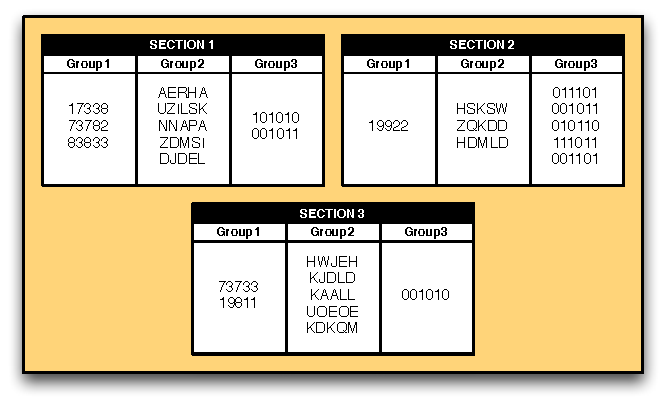
\includegraphics[width=\textwidth]{figures/fig1}
\caption{Example of a structured bulletin board with three sections, three groups, and corresponding messages.}
\label{fig1}
\end{figure}

%-----------------------------------------------------------------------------------------------
\paragraph*{Property 3: Typed.}
%-----------------------------------------------------------------------------------------------
A grouped bulletin board is called \emph{typed}, if each group $g_i\in\mathcal{G}$ defines its own set  $\mathcal{M}_i\subseteq \mathcal{M}$ of valid messages. $\mathcal{M}_i$ is called \emph{type} of $g_i$.  In a typed board, an incoming messages $m$ for group $g_i$ is accepted if $m\in\mathcal{M}_i$, and all other messages are rejected. The example of \Cref{fig1} shows a typed board with different types of messages for each group, for example $\mathcal{M}_1=\{0,\ldots,9\}^5$, $\mathcal{M}_2=\{A,\ldots,Z\}^5$, $\mathcal{M}_3=\{0,1\}^6$.

%-----------------------------------------------------------------------------------------------
\paragraph*{Property 4: Access-Controlled.}
%-----------------------------------------------------------------------------------------------

In certain applications, only a well-defined set of users is authorized to post messages to the bulletin board. A bulletin board is called \emph{access-controlled}, if it provides an access-control mechanism that identifies the author of a message and rejects the message if the user is unauthorized. To enable the board doing this check, we assume that a set $\mathcal{K}$ of public signature keys---one for each authorized user---is known to the board at every moment. This set is either \emph{static} or \emph{dynamic}, depending on whether the set of authorized users is fixed or can change over time. In the static case, $\mathcal{K}$ is publicly known and can not be changed, whereas in the dynamic case, $\mathcal{K}=K(\mathcal{P}, \alpha, t)$ is defined implicitly by a publicly known function $K$, where $\mathcal{P}$ is the current set of posts published on the board, $\alpha$ the list of user attributes accompanying the message, and $t$ the current time. The arguments of $K$ are optional, i.e., not all three of them are relevant in every case. For a message $m$ to be accepted by the board, it must be signed by the user using a private signature key $sk$ for a public key in $vk\in\mathcal{K}$. The signature $S_m=\mathit{sign}_{sk_U}(m, \alpha_I)$ and the public key $vk$ are included in the post as user attributes. The board can then perform the checks $vk\in\mathcal{K}$ and $\mathit{verify}_{\vk{}}(m,\alpha_I,S_m)$ to decide if the user of $m$ is authorized.

%-----------------------------------------------------------------------------------------------
\paragraph*{Property 5: Ordered.}
%-----------------------------------------------------------------------------------------------

The ordered property ensures that all published posts $\mathcal{P}_{\langle s\rangle}$ for a section have a total order. This is achieved by adding a sequence number $n\in\mathbb{N}$ to $\beta$ for the post, where $n=|\mathcal{P}_{\langle s\rangle}|+1$.

%-----------------------------------------------------------------------------------------------
\paragraph*{Property 6: Chronological.}
%-----------------------------------------------------------------------------------------------

A chronological board adds to every incoming message a timestamp $t\in\mathcal{T}$ into $\beta$, which denotes when the message was received by the board.

%-----------------------------------------------------------------------------------------------
\paragraph*{Property 7: Append-Only.}
%-----------------------------------------------------------------------------------------------

The append-only property ensures that no posted message can be removed from the board or be changed. So, $\mathcal{P}_{\langle t\rangle} \subseteq \mathcal{P}_{{\langle t+1\rangle}}$ where $\mathcal{P}_{{\langle t\rangle}} $ represent the content on the board at time $t$. The solution presented here requires that the board has the ordered property. The board creates a hash-chain $H_s$ over $\mathcal{P}_{\langle s\rangle}$. For each $p_i$ it creates a hash $h_i\in{H_s}$ which is the result of the hash function $\mathit{Hash}(h_{i-1}, p_i, \alpha, \beta_{I})$, where $h_{i-1}$ is the hash of the preceding post $p_{i-1}$ and $h_0=0$.
This hash $h_i$ is then added to $\beta$.

%-----------------------------------------------------------------------------------------------
\paragraph*{Property 8: Certified Posting.}
%-----------------------------------------------------------------------------------------------

With certified posting every user receives after a successful post a receipt from the board, which confirms that the message has been published.
Upon posting a message $m$, the board creates the signature $S_p= Sign_{sk_{BB}}(m, \alpha,\beta_I)$ including the message, and the user attributes and a sub set of the board attributes $\beta_I$. This signature is added to $\beta$.

%===============================================================================================
\section{Query Properties}\label{ub3}
%===============================================================================================

\paragraph*{Property 9: Certified Reading.}

This property forces the board to commit to every result $R$ it returns. This is achieved by adding a timestamp $t$ and a signature $S_q=Sign_{sk_{BB}}(Q, R, \gamma_I)$ to $\gamma$.

%===============================================================================================
\section{Further Properties}
%===============================================================================================

\paragraph*{Property 10: Notifying.}

The notification property of the board allows an entity  $e$ to register itself to be notified when a certain set of messages $\mathcal{P}(Q)$ is posted on the board. In order to accomplish that, two additional methods must be introduced:

\begin{itemize}
	\item Register$(e, Q): c$ \newline Where $Q$ represents the query for the messages the entity is interested in and $c$ a notification code, which can be used to unregister. 
	\item Unregister$(c):-$ \newline By providing his/her notification code $c$, one can unregister and will not receive any further notification.
\end{itemize}

%===============================================================================================
\section{Properties of UniVote and UniCert}\label{ub4}
%===============================================================================================

For UniVote and UniCert a bulletin board that supports all properties described in the previous sections is used. This results in our UniBoard configuration supporting following four operations. Also note that Schnorr signatures are used for signing. Therefore every sign operation needs an additional random value $r$ (Chapter \ref{schnorrsig}).

\subsection{Post}
 $\mathrm{Post}(m, (s, g, S_m, vk)):(n, t , h, S_p)$
\begin{enumerate}
	\item Check that section $s$ exists.
	\item Check that group $g$ exists.
	\item Check if message $m$ is of the type of group $g$.
	\item Check that $S_m$ is a correct signature of $(m, (s, g))$ and belongs to $vk$.
	\item Check that $k$ is authorized by checking $\mathcal{K}$.
	\item Define the total order $n$ of the message in $s$ .
	\item Add the current time $t$ to the message.
	\item Create the hash $h$ for the message.
	\item Create the signature for the post $S_p=Sign_{sk_{BB}}(m, (s, g, S_m , vk), (n, t, h))$
	\item Send notifications for this message if necessary.
	\item Save the post.
	\item Return $(n, t, h, S_p)$ to the user.
\end{enumerate}

A user can use the compact notation $\mathrm{Post}(m, s, g)$, which represents the following three steps:
\begin{enumerate}
	\item Create the Schnorr signature $S_m=\mathit{sign}_{sk_U}((m,(s,g)),r)$
	\item Post the message on the board $\mathrm{Post}(m, (s, g, S_m, vk))$
	\item Validate and save the response $(n, t , h, S_p)$.
\end{enumerate}

\subsection{Query}
For the get operation the query is  $Q\subseteq\mathcal{M}\times\mathcal{S}\times\mathcal{G}\times\Sigma_a\times\mathcal{K}\times\mathbb{N}\times\mathcal{T}\times\mathcal{H}\times\Sigma_p$. \newline\newline
$\mathrm{Get}(Q): R, (t, S_Q)$
\begin{enumerate}
	\item Search all messages $\mathcal{P}_Q$ satisfying $Q$.
	\item Set timestamp $t$ to the current time.
	\item Create the signature $S_Q$.
	\item return the result to the reader.
\end{enumerate}
$\mathrm{Register}(e, Q): c$
\begin{enumerate}
	\item Generate a unique notification code $c$.
	\item Save the notification and the notification code
	\item Return $c$.
\end{enumerate}
$\mathrm{Unregister}(c): -$
\begin{enumerate}
	\item Check if there is notification active, that corresponds to the notification code $c$.
	\item Remove the notification.
\end{enumerate}

\paragraph*{Multiple instances}
As there can be multiple instances of UniBoard running, they need to be recognisable. This is achieved by denoting every operation with an application identifier , e.g. $\mathrm{Post}_{UV}(m,\alpha):\beta$ for UniVote 
%This property is completely on the operational level as the bulletin board for each application $l$ is independent. This property allows one UniBoard instance to provide service to multiple applications. This is achieved by adding the application $l$ to every operation provided by UniBoard, e.g. $\mathrm{Post}_l(m,\alpha):\beta$.


%===============================================================================================
\chapter{UniCert}
%===============================================================================================

UniCert is a certification authority, that issues digital certificates used to authenticate users, to sign and/or encrypt messages. UniCert provides an interface where the user can authenticate themselves and request a certificate corresponding to their needs. UniCert uses UniBoard to publish all issued certificates.

\paragraph*{Authentication} A digital certificate must be linked to an entity, thus the entity has to authenticate itself to UniCert. Authentication in UniCert can be done via various identity providers (e.g. SwitchAAI, Google, ...). The user has to authenticate themselves against one of these providers which returns the resulting \emph{authentication token} $t_{auth}$ to UniCert. The form and content of the token can be different depending on which identity provider is used. However, it must contain at least one value allowing to uniquely identify the user among all users of this identity provider.
%UniCert then verifies if the identity received corresponds to the information that are asked to figure in the certificate. If yes, a certificate can be issued using the public key and usage field (see next section) provided. 
UniCert then issues a certificate based on the identity information present in the token and on other properties provided by the requester.  Therefore, UniCert uses a function $\mathit{f}(t_{auth})$, to extract the needed information from the authentication token, resulting in a identifier $id$. $\mathit{f}$ must use at least one unique identifier present in the token in order to be able to output different results for two different inputs. UniCert defines a set $\mathcal{F}$ of functions $\mathit{f}$ allowing to select information from the authentication token, or to make some processing on them before putting them in the certificate (e.g anonymization by using a one-way function). The user has to choose one of the functions provided by UniCert. A reference to the identity provider used is inserted in the certificate.


\paragraph*{Application Identifier and Role} A user should have the possibility to request multiple certificates. This allows them to manage them differently. For example, they can use a certificate for critical tasks and another one for less critical tasks. The way the user manages the private keys of these two certificates is certainly different. In order make it possible for the user to request multiple certificates, there must be a way to distinguish them. In some cases, this could be done using the cryptographic values in the certificate\footnote{For example different p, q and generators in discrete logarithm certificates.} but this is not always possible.\footnote{For example in RSA certificates: $e,n$ is always different and thus it cannot be defined that such setup is for such task} Therefore, two additional fields are added to the certificate: an \textit{application identifier} $a$ and a \textit{role} $r$. The application identifier allows the user to request certificates for different applications. The application where the certificate is used can (but does not have to) check this field if necessary. The role allows to distinguish certificates issued for the same application. This way, the user can use different certificates for different purposes inside the same application. So, if an application wants to use roles, it has to define them. $a$ and $r$ are both strings. The pair ($a$, $r$) should be unique among all applications, but UniCert cannot ensure that fact since it does not know all applications.

\paragraph*{Certificate revocation} Certificates are not explicitly revoked. An application can consider a certificate as implicitly revoked if a newer one has been issued for the same user, the same application identifier $a$, the same role $r$ and the same identity provider.

%Each application using UniCert should be able to personalize some content of the certificates in order to differentiate the certificates more easily. Therefore, the requester must provide an application identifier $a$ that will be included in the certificate. By default, this value is an empty string. The application identifiers are not know in advance by UniCert since it does not necessarily know the applications for which it issues certificates.

%An application could require the user to have multiple certificates for different purposes. Thus, the application must be able to differentiate them. To allow this, the certificate requester must indicate a \emph{role} $r$ when requesting the certificate to UniCert. The role is a number in $\mathbb{N}$ that can be interpreted differently by each application. The default value is 0. The pair ($a$, $r$) should be unique among all applications, but UniCert cannot ensure that fact since it does not know all applications.

%Each issued certificate can be used for a specific purpose also called \emph{Role} (e.g. voter certificate, tallier certificate, ...) which is mentioned in the certificate. This field can be used in the application to identify the certificate more easily. This field must be an number, it is however not a mandatory field. In order to have unique roles identifiers across all applications, the role number is concatenated with an application identifier. The application identifier should be unique among all applications. These identifiers are not know in advance by UniCert since it does not necessarily know the applications for which it issues certificates. These applications identifiers are hashed before being combined with the role, in order to avoid publication of undesirable texts in the certificates.

%the usage is linked to a given cryptographic setup (e.g specific $p,q$ and $g$ values for a DSA certificate, a prime size) and other properties (e.g. privacy properties) . When requesting a certificate, the requester must indicate a usage and compute a private key corresponding to the setup linked with the selected usage. The usage is mentioned in a critical extension of the X.509 certificate issued.

%\paragraph*{Data privacy} Since the issued certificates are published on UniBoard, one could want the certificates to be anonymized. This requirement must be provided to UniCert when requesting the certificate. This is done by providing a function $f(\mathit{id})$ that must be applied to the content of the authentication token. The result of this function is used as distinguished name in the certificate. For example, instead of just using the mail address present in the $t_{auth}$, the requester can provide a function that hashes mail address.

\paragraph*{Certificate generation procedure} The involved parties in certificate generation procedure are UniCert (\UC), the user $\User$ requesting the certificate, the UniBoard instance (\UBC), and the identity providers $\IdentityProvider\in\mathcal{I}$ supported by \UC. The process works as follows:

\begin{enumerate}
	\item $\User$ chooses the following parameter: cryptographic setup $s$, function $\mathit{f} \in \mathcal{F}$, identity provider $\IdentityProvider \in \mathcal{I}$, application identifier $a$, role $r$.
	\item $\User$ requests an authentication token $t_{auth}$ to one $\IdentityProvider$ and provides the required credentials
\end{enumerate} 

\textit{Keys preparation and certificate request}
\begin{enumerate}[resume]
	\item Using $s$, $\User$ generates a private key $x$ and compute the corresponding public key $y$
	\item $\User$ signs the data sent to \UC to prove knowledge of $x$: $S_{req} = \mathit{sign}_{x}(s, y, t_{auth},\mathit{f}, I, a, r)$.\footnote{ElGamal encryption keys cannot properly be used to generate a signature. Thus, in case the user request a discrete logarithm certificate, a zero knowledge proof of knowledge of $x$ replaces the signature. The other values used in the signature would be injected in the hash function of the non-interactive proof in order to also provide a commitment to these other values.}
	\item $\User$ sends $s$, $y$, $t_{auth}$, $\mathit{f}$, $\IdentityProvider$, a, r, $S_{req}$ to \UC
\end{enumerate} 

%\textit{Authentication}
%\begin{enumerate}[resume]
%	\item $UC$ generates an authentication request $t_{req}$ for $R$ to $I_i$
%	\item $R$ authenticate themselves to $I_i$
%	\item If authentication was successful, $I_i$ generates an authentication response $t_{auth}$ for $R$ in form of a token
%	\item $R$ transfers $t_{auth}$ to \UC
%\end{enumerate} 

\textit{Certificate creation}
\begin{enumerate}[resume]
	\item \UC checks if $a$, $r$, $\IdentityProvider$ and $\mathit{f}$ are value of their respective set
	\item \UC checks if $t_{auth}$ is valid
	\item \UC checks the validity of the cryptographic setup $s$
	\item \UC verifies $S_{req}$ with $y$
	%\item \UC checks on \UBC if $\User$ already owns a certificate with the same role $r$ for application $A$. If yes, \UC revokes it.
	\item \UC generates the identifier $id$ for $\User$ using $\mathit{f}$ and $t_{auth}$
	\item \UC generates the certificate $Z_{U}=\mathit{csertify}_{\SK{\UC}}(id,y,t, s,a,r,I)$ where $t$ is a timestamp
	\item \UC posts $(\mathit{certificates}: Z_{U})$ to \UBC
	\item \UC returns $Z_{U}$ to $\User$
\end{enumerate} 	
		
	
%	\item \UC gets the available usages $\mathcal{U}$ from \UBC \todo{get()} \todo{From where are the "usage" possibilities read? From each section for UniVote in UniBoard? => read over multiple sections... Theoretically not, because the setup is not related to an election but to a group of elections.}  \todo{Who defines the usages? The Election Coordinator?}
%	\item $R$ chooses a usage $u$ in $\mathcal{U}$ proposed by \UC 
%	\item $R$ gets the cryptographic setup $s$ corresponding to $u$ from \UBC \todo{get() }\todo{How is the link between crypto setup and usage done? And what about other properties?}
%
%	\item $R$ generates a private key $x$ with $s$ and compute the corresponding public key $y$
%	\item $R$ compute a zero knowledge proof $\pi$ showing that they know $x$
%	\item $R$ sends $y$, $\pi$ and $u$ to \UC \todo{Format of the public key to submit?}
%	 if $R$ is authorized to generate a certificate for $u$ \todo{is it needed? If yes, how is that done?}
%	
%	
%	\item \UC checks if $s$ used by $R$ to generate $x$ and $y$ is the same as $s'$ corresponding to $u$
%	\item \UC get the properties $\mathcal{P}$ linked to $u$ from \UBC \todo{get()}
%	\item \UC checks on \UBC if there exists already a certificate for $R$ with the same $u$. If yes, \UC revokes it.
%	\item \UC generates the certificate $c$ using $a_{resp}$, $y$, $u$ and $\mathcal{P}$ \todo{Format of the certificate?} \todo{Describe which field of X.509 certificate contains what?} \todo{Which hash method is used for DN?}
%	\item \UC publishes $c$ on \UBC and returns $c$ to $R$


%\subsubsection{Registration Renewal}
%The above procedure allows $\Voter{i}$ to renew the registration at any time, simply by performing the same steps again. The new certificate $\bar{Z}_i=(\Voter{i},\vkbar{i},\bar{t}_i,\CA,\bar{S}_i)$ will contain a timestamp $\bar{t}_i>t_i$, which will implicitly disqualify any former certificate $Z_i=(\Voter{i},\vk{i},t_i,\CA,S_i)$ in current or future elections. \CA should warn $\Voter{i}$ before issuing a new certificate.

\paragraph*{UniCert and UniBoard} As already said, UniCert publishes the issued certificates on UniBoard. Therefore, UniCert must define the different parameter required by UniBoard when posting and getting messages.

\begin{itemize}
	%\item $\mathcal{S}$: one section is needed per application requesting certificate. In this case, only UniVote will use UniCert so $\mathcal{S} = \{\text{"univote"}\}$
	\item $\mathcal{S}$: only one section is used to publish all certificates by UniCert. This avoids that a new section has to be created each time a new application identifier is used. So, $\mathcal{S} = \{\text{"unicert"}\}$
	\item $\mathcal{G}$: one group is needed for stocking the issued certificates. So, $\mathcal{G} = \{\text{"certificates"}\}$
	\item $\mathcal{K} = \{k_{\UC}\}$
	\item $\mathcal{M}_{certificates}$: Format of a certificate.
\end{itemize}

%First of all, the requester has to authenticate themselves against an identity provider. The authentication token returned is transmitted to UniCert. Then, the requester has to select the usage for which the certificate must be emitted. Then, they have to generate the private key and the corresponding public key with the setup linked to the selected usage. The usage and the public key can then be provided to UniCert.

%Before creating the certificate with the information submitted by the requester, UniCert has to verify some properties:
%\begin{itemize}
%	\item check if the authentication was successful
%	\item check if this entity is allowed to create a certificate for the selected usage
%	\item check if the cryptographic setup used to generate the private and public keys matches the one specified by the selected usage
%	\item check if the requester knows the private key corresponding to the public one submitted
%	\item check if the distinguished name of the requester must be a hash of the mail address or the mail address itself
%\end{itemize}

%When all these verifications succeed, the certificate is generated with the submitted information and the information present in the authentication token. Finally, the certificate is published on UniBoard and returned to the requester.


%===============================================================================================
\chapter{UniVote}
%===============================================================================================

%===============================================================================================
\section{Overview}
%===============================================================================================


%-----------------------------------------------------------------------------------------------
\subsection{Involved Parties}
%-----------------------------------------------------------------------------------------------

\begin{description}
	\item[UniCert.] \UC
	\item[Election Administration.] \EA
	\item[Election Coordinator.] \EC
	\item[UniBoard (UniVote)] \UBV
	\item[UniBoard (UniCert)] \UBC
	\item[Talliers.] $T=\{\Tallier{1},\ldots,\Tallier{t}\}$
	\item[Mixers.] $M=\{\Mixer{1},\ldots,\Mixer{m}\}$
	\item[Voters.] $V=\{\Voter{1},\ldots,\Voter{n}\}$
\end{description}

Number of ballots: $N\leq n$

%-----------------------------------------------------------------------------------------------
\subsection{Voting Process}
%-----------------------------------------------------------------------------------------------

%-----------------------------------------------------------------------------------------------
\subsection{Public Identifiers and Keys}
%-----------------------------------------------------------------------------------------------

Certificates for the following identifiers are assumed to be publicly known.

Bulletin Board (UniVote):
\begin{itemize}
	\item Identifier: \UBV
	\item Public certificate: $Z_{\UBV}$, signed by \CA at time $t$
	\item Public verification key: $\VK{\UBV}$ 
	\item Private signature key: $\SK{\UBV}$
\end{itemize}

Bulletin Board (UniCert):
\begin{itemize}
	\item Identifier: \UBC
	\item Public certificate: $Z_{\UBC}$, signed by \CA at time $t$
	\item Public verification key: $\VK{\UBC}$ 
	\item Private signature key: $\SK{\UBC}$
\end{itemize}


UniCert:
\begin{itemize}
	\item Identifier: \CA
	\item Public certificate: $Z_{\CA}$, self-signed or certified by public certification authority at time $t$
	\item Public verification key: $\VK{\CA}$
	\item Private signature key: $\SK{\CA}$
\end{itemize}


Certificates for the following identifiers are assumed to be available on \UBC.


Election Coordinator:
\begin{itemize}
	\item Identifier: \EC
	\item Public certificate: $Z_{\EC}$, signed by \CA at time $t$
	\item Public verification key: $\VK{\EC}$ 
	\item Private signature key: $\SK{\EC}$
\end{itemize}

Election Administration:
\begin{itemize}
	\item Identifier: \EA
	\item Public certificate: $Z_{\EA}$, signed by \CA at time $t$
	\item Public verification key: $\VK{\EA}$ 
	\item Private signature key: $\SK{\EA}$
\end{itemize}

Talliers: (for $1\leq j\leq r$)
\begin{itemize}
	\item Identifier: $\Tallier{j}$
	\item Public certificate: $Z_{j}$, signed by \CA at time $t_j$
	\item Public verification key: $\vk{j}$ 
	\item Private signature key: $\sk{j}$
\end{itemize}

Mixers: (for $1\leq k\leq m$)
\begin{itemize}
	\item Identifier: $\Mixer{k}$
	\item Public certificate: $Z_{k}$, signed by \CA at time $t_k$
	\item Public verification key: $\vk{k}$ 
	\item Private signature key: $\sk{k}$
\end{itemize}

Voters: (for $1\leq i\leq n$)
\begin{itemize}
	\item Identifier: $\Voter{i}$
	\item Personal credentials: $\cred{i}$ issued by the \CA or an affiliated identity provider.
\end{itemize}

%-----------------------------------------------------------------------------------------------
\subsection{Posting and Getting Messages}
%-----------------------------------------------------------------------------------------------

Post involves signature and section id

Get involves checking the signature

%===============================================================================================
\section{Detailed Protocol Specification}
%===============================================================================================



%-----------------------------------------------------------------------------------------------
\subsection{Election Setup}
%-----------------------------------------------------------------------------------------------

The following tasks can be performed in advance, possibly long before the election starts.

\subsubsection{Initialization}

\EA requests from \EC to run an election. \EC chooses a unique election identifier $\eid$ and requests from \UBV the initialization of the election. \UBV performs the following steps: 
\begin{enumerate}
	\item Initialize a new section with identifier $\eid$.
	\item Define \EC to become the section coordinator.
\end{enumerate}

\EC performs the following steps: 
\begin{enumerate}[resume]
	\item Get $(\textsf{certificate}:Z_{\EA})$ from \UBC, where $Z_{\EA}$ is the most recent UniVote election administration certificate.
	\item Verify $Z_{\EA}$.
	\item Post $(\mathsf{administrationCertificate}: Z_{\EA})$ to \UBV.
\end{enumerate}

\subsubsection{Election Definition}
\EC performs the following steps: 
\begin{enumerate}
	\item Select $\vk{\EA}$ from $Z_{\EA}$.
	\item Post $(\mathsf{accessRight}: \vk{\EA}, \mathsf{electionDefinition}, 1)$ to \UBV.
	\item Post $(\mathsf{accessRight}: \vk{\EA}, \mathsf{trustees}, 1)$ to \UBV.
	\item Post $(\mathsf{accessRight}: \vk{\EA}, \mathsf{securityLevel}, 1)$ to \UBV.
\end{enumerate}
\EA performs the following steps: 
\begin{enumerate}[resume]
	\item Define textual description $\descrElection$ of the election event (title, description, election rules, languages, etc.).
	\item Define $\period =(t_{1},t_{2})$.
	\item Post $(\mathsf{electionDefinition}: \descrElection,\period)$ to \UBV.
	\item Define talliers $T=\{\Tallier{1},\ldots,\Tallier{t}\}$.
	\item Define mixers $M=\{\Mixer{1}\ldots,\Mixer{m}\}$.
	\item Post $(\mathsf{trustees}: T, M)$ to \UBV.
	\item Select $\security\in\{1,2,3\}$
	\item Post $(\mathsf{securityLevel}: \security)$ to \UBV.
\end{enumerate}
\EC performs the following steps:
\begin{enumerate}[resume]
	\item Get $(\mathsf{trustees}: T, M)$ from \UBV.
	\item For each $\Tallier{j}\in T$:
	\begin{enumerate}
		\item Get $(\textsf{certificate}:Z_{j})$ from \UBC, where $Z_j$ is the most recent UniVote tallier certificate.
		\item Verify $Z_{j}$.
	\end{enumerate}
	Let $\mathcal{Z}_{T}=\{Z_j:1\leq j\leq r\}$  denote the corresponding set of certificates.
	\item For each $\Mixer{k}\in M$:
	\begin{enumerate}
		\item Get $(\textsf{certificate}:Z_{k})$ from \UBC, where $Z_k$ is the most recent UniVote mixer certificate.
		\item Verify $Z_{k}$.
	\end{enumerate}
	Let $\mathcal{Z}_{M}=\{Z_k:1\leq k\leq m\}$ denote the corresponding set of certificates.
	\item Post $(\mathsf{trusteeCertificates}: \mathcal{Z}_{T},\mathcal{Z}_{M})$ to \UBV.
\end{enumerate}

\subsubsection{Cryptographic Setting}

\EC performs the following steps:
\begin{enumerate}
	\item Get $(\mathsf{securityLevel}: \security)$ from \UBV.
	\item Select 
	\begin{itemize}
		\item $\mathit{encSetting}\in \Sigma_\mathsf{ENC}$, 
		\item $\mathit{sigSetting}\in \Sigma_\mathsf{SIG}$, 
		\item $\mathit{hashSetting}\in \Sigma_\mathsf{HASH}$ 
	\end{itemize}
	according to $\security$, where $\Sigma_\mathsf{ENC}$, $\Sigma_\mathsf{SIG}$, $\Sigma_\mathsf{HASH}$ are corresponding sets of predefined cryptographic settings for ElGamal encryptions, Schnorr signatures, and hash functions, respectively (see \Cref{settings}).
	\item Post $(\mathsf{cryptoSetting}:\mathit{encSetting},\mathit{sigSetting},\mathit{hashSetting})$ to \UBV.	
\end{enumerate}

\subsubsection{Shared Encryption Key}
	
For each $Z_{j}\in \mathcal{Z}_{T}$, \EC performs the following steps:
\begin{enumerate}	
	\item Select $\vk{j}$ from $Z_{j}$.
	\item Post $(\mathsf{accessRight}:\vk{j},\mathsf{encryptionKeyShare},1)$ to \UBV.
\end{enumerate}

Each $\Tallier{j}\in T$ performs the following steps:
\begin{enumerate}[resume]
	\item Get $(\mathsf{cryptoSetting}:\mathit{encSetting},\mathit{sigSetting},\mathit{hashSetting})$ from \UBV.
	\item Retrieve $\mathcal{G}_Q$ and $G$ from $\mathit{encSetting}$.
	\item Choose $x_j\in_R\mathbb{Z}_Q$.
	\item Compute $y_j = G^{x_j}$.
	\item Generate $\pi_{j}=\mathit{NIZKP}\{(x_j):y_j=G^{x_j}\}$.
	\item Post $(\mathsf{encryptionKeyShare}:y_j,\pi_{j})$ to \UBV.
\end{enumerate}

\EC performs the following steps:
\begin{enumerate}[resume]
	\item For each $\Tallier{j}\in T$:
	\begin{enumerate}
		\item Get $(\mathsf{encryptionKeyShare}:y_j,\pi_{j})$ from \UBV.
		\item Verify $\pi_{j}$.
	\end{enumerate}
	\item Compute $y=\prod_j y_j$.
	\item Post $(\mathsf{encryptionKey}:y)$ to \UBV.
\end{enumerate}


%-----------------------------------------------------------------------------------------------
\subsection{Election Preparation}\label{preparation}
%-----------------------------------------------------------------------------------------------

The following tasks are performed shortly before starting the election.

\subsubsection{Definition of Election Options and Electoral Roll}

\EC performs the following step:
\begin{enumerate}
	\item Post $(\mathsf{accessRight}: \vk{\EA}, \mathsf{electionOptions}, 1)$ to \UBV.
	\item Post $(\mathsf{accessRight}: \vk{\EA}, \mathsf{electoralRoll}, 1)$ to \UBV.
\end{enumerate}

\EA performs the following steps:
\begin{enumerate}[resume]
	\item Define the set of choices $C=\{c_1,\ldots,c_s\}$ and a rule set $R$ describing the set $\mathcal{W}=\mathit{electionOptions}(C,R)$ of valid \emph{election options}, where $\mathit{electionOptions}$ is a publicly known function (see \secref{choices} for details).
	\item Define a detailed description $\descrOptions$ of the election options (election type, lists of choices, etc.).\footnote{This information is only relevant for presenting the election choices and options to the voter.}
	\item Post $(\mathsf{electionOptions}:C,R,\descrOptions)$ to \UBV.
	\item Define the \emph{electoral roll} $V=\{\Voter{1},\ldots,\Voter{n}\}$.
	\item Post $(\mathsf{electoralRoll}:V)$ to \UBV.
\end{enumerate}

\EC performs the following steps:
\begin{enumerate}[resume]
	\item Get  $(\mathit{electoralRoll}:V)$ from \UBV.
	\item For every $V_i\in V$:
	\begin{itemize}
		\item Get $(\mathsf{certificate}:Z_i)$ from \UBC, where $Z_i$ is the most recent UniVote voter certificate for $\mathit{sigSetting}$.
		\item Verify $Z_i$.
	\end{itemize}
	Let $\mathcal{Z}_V=\{Z_1,\ldots,Z_{n}\}$ denote the set of valid voter certificates.\footnote{To simplify the notation, we assume that $|V|=|\mathcal{Z}_V|=n$. In general, the number of valid certificates will be smaller or equal than the number of eligible voters.}
	\item Post $(\mathsf{voterCertificates}:\mathcal{Z}_V)$ on \UBV.
\end{enumerate}


\subsubsection{Mixing the Public Keys}
\EC performs the following steps:
\begin{enumerate}
	\item Select $\mathit{VK}_0=\{\vk{1},\ldots,\vk{n}\}$ from $\mathcal{Z}_V$.
	\item Let $g_0=g$.
\end{enumerate}
The following steps are repeated for every $\Mixer{k}\in M$ (in ascending order for $1\leq k\leq m$):
\begin{enumerate}[resume]
	\item \EC performs the following steps:
	\begin{enumerate}
		\item Post $(\mathsf{keyMixingRequest}:\Mixer{k},g_{k-1}, \mathit{VK}_{k-1})$ to \UBV.
		\item Select $\vk{k}$ from $Z_{k}\in \mathcal{Z}_{M}$.
		\item Post $(\mathsf{accessRight}:\vk{k},\mathsf{keyMixingResult},1)$ to \UBV.
	\end{enumerate}
	\item $\Mixer{k}$ performs the following steps:
	\begin{enumerate}
		\item Get $(\mathsf{cryptoSetting}:\mathit{encSetting},\mathit{sigSetting},\mathit{hashSetting}$ from \UBV.
		\item Retrieve $G_q$ and $g$ from $\mathit{sigSetting}$.
		\item Get $(\mathsf{keyMixingRequest}:\Mixer{k}, g_{k-1}, \mathit{VK}_{k-1})$ from \UBV.
		\item Choose $\alpha_k\in_R\mathbb{Z}_q$.
		\item Compute $g_k = g_{k-1}^{\alpha_k}$.
		\item Choose $\psi_k:[1,n]\rightarrow[1,n]\in_R\Psi_n$.
		\item Compute $\mathit{VK}_k=\mathit{shuffle}_{\psi_k}(\mathit{VK}_{k-1},\alpha_k)$.
		\item Generate $\pi_{k}=\mathit{NIZKP}\{(\psi_k,\alpha_k):g_k=g_{k-1}^{\alpha_k}\wedge \mathit{VK}_{k}=\mathit{shuffle}_{\psi_k}(\mathit{VK}_{k-1},\alpha_k)\}$.
		\item Post $(\mathsf{keyMixingResult}:g_k,\mathit{VK}_k,\pi_{k})$ to \UBV.
	\end{enumerate}
	\item \EC performs the following steps:
	\begin{enumerate}
		\item Get $(\mathsf{keyMixingResult}:g_k,\mathit{VK}_k,\pi_{k})$ from \UBV.
		\item Verify $\pi_{k}$.
	\end{enumerate}
\end{enumerate}

Let $\hat{g}=g_m$ denote the \emph{signature generator} for this election and $\hat{\mathit{VK}}=\mathit{VK}_m$ the set of mixed public keys. 

\subsubsection{Finalizing Election Preparation}

\EC performs the following steps:
\begin{enumerate}
	\item Post $(\mathsf{mixedKeys}:\hat{\mathit{VK}})$ to \UBV.
	\item For every $\vkhat{i}\in \hat{\mathit{VK}}$, post $(\mathsf{accessRight}:\vkhat{i}, \mathsf{ballot}, 1,\period)$.
	\item Get $(\mathsf{electionDefinition}: \descrElection,\period)$ from \UBV.
	\item Get $(\mathsf{electionOptions}:C,R,\descrOptions)$ from \UBV.
	\item Post $(\mathsf{electionData}:\descrElection, \period, C, R, \descrOptions, \mathit{encSetting},\mathit{sigSetting},\mathit{hashSetting},y, \hat{g})$ to \UBV.\footnote{This post is only for improved convenience. It contains all the relevant information for casting a vote. Retrieving this information in a single step is the purpose of this post.}
\end{enumerate}

%-----------------------------------------------------------------------------------------------
\subsection{Election Period}\label{election_period}
%-----------------------------------------------------------------------------------------------

\subsubsection{Vote Creation and Casting}

$\Voter{i}\in V$ performs the following steps:
\begin{enumerate}
	\item Get $(\mathsf{electionData}:\descrElection, \period, C, R, \descrOptions, \mathit{encSetting},\mathit{sigSetting},\mathit{hashSetting},y, \hat{g})$ from \UBV.
	\item Retrieve $\mathcal{G}_Q$ and $G$ from $\mathit{encSetting}$.
	\item Retrieve $G_q$ from $\mathit{sigSetting}$.
	\item Choose $v_i\in\mathit{electionOptions}(C,R)$.
	\item Compute $m_i'=\mathit{encode}_{C,R}(v_i) \in \mathbb{Z}_Q$.
	\item Compute $m_i=\mathit{subGroup}(m_i') \in \mathcal{G}_Q$.
	\item Choose $r_i\in_R\mathbb{Z}_Q$.
	\item Compute $E_i=\mathit{encrypt}_y(m_i,r_i)\in\mathcal{G}_Q\times\mathcal{G}_Q$.
	\item Generate $\pi_{i}=\mathit{NIZKP}\{(m_i,r_i):E_i=\mathit{encrypt}_y(m_i,r_i)\}$.\footnote{Note that if $E=(a,b)=(G^{r},m\cdot y^{r})$ is an ElGamal encryption, then $\mathit{NIZKP}\{(m,r):E=\mathit{encrypt}_y(m,r)\}$ is equivalent to $\mathit{NIZKP}\{(r):a=G^{r}\}$, which implies knowledge of $m$.}
	\item Compute $\vkhat{i}=\hat{g}^{\sk{i}}\in\hat{\mathit{VK}}$.
	\item Post $(\mathsf{ballot}:E_i,\pi_{i})$ to \UBV using $\vkhat{i}$.
\end{enumerate}

\subsubsection{Finalizing Election Period}

When the election period is over, \EC performs the following steps:
\begin{enumerate}
	\item Get $(\mathsf{ballot}:\mathcal{B})$ from \UBV.\footnote{Using an extensive check.}
	\item For every $B_i=(E_i,\pi_{i})\in\mathcal{B}$:
		\begin{enumerate}
			\item Verify $\pi_{i}$.
			\item If $\pi_{i}$ is valid, collect $E_{i}$.
		\end{enumerate}
\end{enumerate}
Let $\mathcal{E}_0=\{E_1,\ldots,E_N\}\in(\mathcal{G}_Q\times\mathcal{G}_Q)^N$ be list of valid encrypted votes for $N\leq n$.

%-----------------------------------------------------------------------------------------------
\subsection{Mixing and Tallying}
%-----------------------------------------------------------------------------------------------

\subsubsection{Mixing the Encrypted Votes}

The following steps are repeated for every $\Mixer{k}\in M$ (in ascending order for $1\leq k\leq m$):
\begin{enumerate}
	\item \EC performs the following steps:
	\begin{enumerate}
		\item Post $(\mathsf{voteMixingRequest}:\Mixer{k},\mathcal{E}_{k-1})$ to \UBV.
		\item Select $\vk{k}$ from $Z_{k}\in \mathcal{Z}_{M}$.
		\item Post $(\mathsf{accessRight}:\vk{k},\mathsf{voteMixingResult},1)$ to \UBV.
	\end{enumerate}
	\item $\Mixer{k}$ performs the following steps:
	\begin{enumerate}
		\item Get $(\mathsf{electionSetting}:\mathcal{G}_Q,G)$ from \UBV.
		\item Get $(\mathsf{voteMixingRequest}:\Mixer{k}, \mathcal{E}_{k-1})$ from \UBV.
		\item Choose $R_k=(r_{k,1},\ldots,r_{k,N})\in_R\mathbb{Z}_Q^N$.
		\item Choose $\tau_k:[1,N]\rightarrow[1,N]\in_R\Psi_N$.
		\item Compute $\mathcal{E}_k=\mathit{shuffle}_{\tau_k}(\mathcal{E}_{k-1},R_k)$.
		\item Generate $\pi'_{k}=\mathit{NIZKP}\{(\tau_k,R_k): \mathcal{E}_k=\mathit{shuffle}_{\tau_k}(\mathcal{E}_{k-1},R_k)\}$.
		\item Post $(\mathsf{voteMixingResult}:\mathcal{E}_k,\pi'_{k})$ to \UBV.
	\end{enumerate}
	\item \EC performs the following steps:
	\begin{enumerate}
		\item Get $(\mathsf{voteMixingResult}:\mathcal{E}_k,\pi'_{k})$ from \UBV.
		\item Verify $\pi'_{k}$.
	\end{enumerate}
\end{enumerate}
Let $\hat{\mathcal{E}}=\mathcal{E}_m$ the set of mixed encrypted votes. 

\subsubsection{Decrypting and Tallying the Votes}

\EC performs the following steps:
\begin{enumerate}	
	\item Post $(\mathsf{mixedVotes}:\hat{\mathcal{E}})$ to \UBV.
	\item For each $Z_{j}\in \mathcal{Z}_{T}$:
	\begin{enumerate}
		\item Select $\vk{j}$ from $Z_{j}$.
		\item Post $(\mathsf{accessRight}:\vk{j},\mathsf{partialDecryption},1)$ to \UBV.
	\end{enumerate}
\end{enumerate}

Each $\Tallier{j}\in T$ performs the following steps:
\begin{enumerate}
	\item Get $(\mathsf{mixedVotes}:\hat{\mathcal{E}})$ from \UBV.
	\item Select $A=(a_1,\ldots,a_N)\in\mathcal{G}_Q^N$ from $\hat{\mathcal{E}}=\{(a_i,b_i):1\leq i\leq N\}$. 

	\item Compute $A_j = (a_{1,j},\ldots,a_{N,j})$ for $a_{i,j} = a_i^{-x_j}\in\mathcal{G}_Q$.
	\item Generate $\pi_{j}'=\mathit{NIZKP}\{(x_j):y_j=G^{x_j} \wedge \left(\bigwedge_i a_{i,j} = a_i^{-x_j}\right)\}$.
	\item Post $(\mathsf{partialDecryption}:A_j,\pi_{j}')$ to \UBV.
\end{enumerate}

\EC performs the following steps:
\begin{enumerate}[resume]
	\item For each $\Tallier{j}\in T$:
	\begin{enumerate}
		\item Get $(\mathsf{partialDecryption}:A_j,\pi_{j}')$ from \UBV.
		\item Verify $\pi_{j}'$.
	\end{enumerate}
	\item For all $1\leq i\leq N$:
	\begin{enumerate}
		\item Compute $m_i=b_i\cdot\prod_j a_{i,j}\in\mathcal{G}_Q$.
		\item Compute $m'_i = \mathit{subGroup}^{-1}(m_i)\in\mathbb{Z}_Q$.
		\item Compute $v_i = \mathit{decode}_{C,R}(m'_i)$.
	\end{enumerate}
	\item For $\mathcal{V}=\{v'_1,\ldots,v'_{N}\}$, let $\mathcal{V}'=\mathcal{V}\cap \mathcal{W}=\{v'_1,\ldots,v'_{N'}\}$ be the list of valid plaintext votes $v'_i=(v'_{i,1},\ldots,v'_{i,s})$, where $v'_{i,j}$ denotes the number of votes for $c_j$.
	\item For each $c_j\in C=\{c_1,\ldots,c_s\}$, compute $r_j =\sum_{j=1}^{N'} v'_{i,j}$.
	\item Post $(\mathsf{decryptedVotes}:\mathcal{V}',\mathit{result})$ to \UBV, where $\mathit{result}=(r_1,\ldots,r_s)$ denotes the \emph{election result}.
\end{enumerate}

%===============================================================================================
\section{Late Voter Certificates}
%===============================================================================================

The previously described protocol requires that all UniVote voter certificates exist prior to an election. In some contexts, however, it will be impossible to enforce the existence of all certificates when the election starts. Eligible voters without a certificate would then be excluded from casting a vote, even if they receive a valid voter certificate during the election. To handle such \emph{late voter certificates}, the following procedure is invoked. Recall that $V$ denotes the electoral roll published on \UBV (see \subsecref{preparation}).

%-----------------------------------------------------------------------------------------------
\subsection{Preparation}
%-----------------------------------------------------------------------------------------------

Upon notification of a newly issued voter certificate $\bar{Z}_i$ for $\Voter{i}$, \EC performs the following steps:
\begin{enumerate}
	\item Check if $\Voter{i}\in V$.
	\item Verify $\bar{Z}_i$.
	\item Post $(\mathsf{newVoterCertificate}:\bar{Z}_i)$ to \UBV. 
\end{enumerate}

%-----------------------------------------------------------------------------------------------
\subsection{Cancelling an Existing Key}\label{cancelling}
%-----------------------------------------------------------------------------------------------

The existence of a new certificate $\bar{Z}_i$ requires \EC to cancel an existing public key (if one exists). For this, \EC performs the following steps: 
\begin{enumerate}
	\item Check if $\mathcal{Z}_V$ contains a voter certificate for $\Voter{i}$. If this is the case, let $Z_i\in\mathcal{Z}_V$ denote this certificate. If this is not the case, discard the following steps and continue with the procedure in \Cref{adding}.
	\item Select $\vk{i,0}$ from $Z_i$.
\end{enumerate}	
The following steps are repeated for every $\Mixer{k}\in M$ (in ascending order for $1\leq k\leq m$):
\begin{enumerate}[resume]
	\item \EC performs the following steps:
	\begin{enumerate}
		\item Post $(\mathsf{keyCancellingRequest}:\Mixer{k}, \Voter{i}, \vk{i,k-1})$ to \UBV.
		\item Select $\vk{k}$ from $Z_{k}\in \mathcal{Z}_{M}$.
		\item Post $(\mathsf{accessRight}:\vk{k},\mathsf{keyCancellingResult},1)$ to \UBV.
	\end{enumerate}
	\item $\Mixer{k}$ performs the following steps:
	\begin{enumerate}
		\item Get $(\mathsf{keyCancellingRequest}: \Mixer{k}, \Voter{i}, \vk{i,k-1})$ from \UBV.
		\item Compute $\vk{i,k} = \vk{i,k-1}^{\alpha_k}$
		\item Generate $\pi_{i,k}=\mathit{NIZKP}\{(\alpha_k):g_k=g_{k-1}^{\alpha_k}\wedge \vk{i,k} = \vk{i,k-1}^{\alpha_k}$.
		\item Post $(\mathsf{keyCancellingResponse}:\Voter{i}, \vk{i,k}, \pi_{i,k})$ to \UBV.
	\end{enumerate}
	\item \EC performs the following steps:
	\begin{enumerate}
		\item Get $(\mathsf{keyCancellingResponse}:\Voter{i}, \vk{i,k}, \pi_{i,k})$ from \UBV.
		\item Verify $\pi_{i,k}$.
	\end{enumerate}
\end{enumerate}
Let $\vkhat{i}=\vk{i,m}$ denote the cancelled anonymized public key. \EC performs the following steps:
\begin{enumerate}
	\item Post $(\mathsf{cancelledKey}:\vkhat{i})$ to \UBV.
	\item Post $(\mathsf{accessRight}:\vkhat{i}, \mathsf{ballot}, 0,\period)$. to \UBV.
\end{enumerate}

%-----------------------------------------------------------------------------------------------
\subsection{Adding the New Certificate}\label{adding}
%-----------------------------------------------------------------------------------------------

\EC performs the following steps:
\begin{enumerate}
	\item Check if $\Voter{i}\in V$.
	\item Get $(\mathsf{certificate}:\bar{Z}_i)$ from \UBC, where $\bar{Z}_i$ is the most recent issued UniVote voter certificate for $\mathit{sigSetting}$.
	\item Post $(\mathsf{newVoterCertificate}:\bar{Z}_i)$ to \UBV. 
\end{enumerate}
Let $\bar{\mathcal{Z}}_V$ denote the current set of certificates added during the election period.

Let $\vkbar{i,0}=\vkbar{i}$ be the new verification key from $\bar{Z}_i$. Repeat the following steps for each $\Mixer{k}\in M$ (in ascending order for $1\leq k\leq m$):\footnote{Note that this procedure corresponds to the borderline case of the general mixing procedure for a single innput public key (with a simplified proof).}
\begin{enumerate}[resume]
	\item Compute $\vkbar{i,k}=\vkbar{i,k-1}^{\alpha_k}$.
\	\item Generate $\pi_{\vkbar{i,k}}=\mathit{NIZKP}\{(\alpha_k):g_k=g_{k-1}^{\alpha_k}\wedge\vkbar{i,k}=\vkbar{i,k-1}^{\alpha_k}\}$.
	\item Post $(\Mixer{k},\eid,\vkbar{i,k},\pi_{\vkbar{i,k}})$ to \UBV.
\end{enumerate}

\EC performs the following steps:
\begin{enumerate}[resume]
	\item For each $\Mixer{k}\in M$, do the following:
	\begin{enumerate}
		\item Check that $\mathit{verify}_{\vk{k}}(\eid,\vkbar{i,k},\pi_{\vkbar{i,k}},S_{\vkbar{k}})=\mathit{accept}$.
		\item Check correctness of $\pi_{\vkbar{i,k}}$ (see \subsecref{proof_reg_new} for details).
	\end{enumerate}
	\item Let $\vkbarprime{i}=\vkbar{i,m}=\vkbar{i}^{\alpha}$.
	\item Post $(\EC,\eid,\Voter{i},\vkbarprime{i})$ to \UBV. Let $\bar{\mathit{VK}}'$ denote the set of all public keys $\vkbarprime{i}$ added during the election period.
\end{enumerate}

%-----------------------------------------------------------------------------------------------
\subsection{Late Renewal of Registration}
%-----------------------------------------------------------------------------------------------

Essentially the same steps are repeated, if the current set $\mathcal{Z}_V \cup \bar{\mathcal{Z}}_V$ contains an earlier certificate $\hat{Z}_i=(\Voter{i},\vkhat{i},\hat{t}_i,\CA,\hat{C}_i)$ of $\Voter{i}$. Note that the first part of the above procedure is not repeated, since $\hat{Z}_i\in\mathcal{Z}_V \cup \bar{\mathcal{Z}}_V$ implies that $\hat{Z}_i$ has already been verified. Let $\vkhat{i,0}=\vkhat{i}$ be the former verification key from $\hat{Z}_i$. Repeat the following steps for each $\Mixer{k}\in M$ (in ascending order for $1\leq k\leq m$):\footnote{Again, this procedure corresponds to the borderline case of the general mixing procedure for a single innput public key (with a simplified proof).}

\begin{enumerate}
	\item Compute $\vkhat{i,k}=\vkhat{i,k-1}^{\alpha_k}$.
\	\item Generate $\pi_{\vkhat{i,k}}=\mathit{NIZKP}\{(\alpha_k):g_k=g_{k-1}^{\alpha_k}\wedge\vkhat{i,k}=\vkhat{i,k-1}^{\alpha_k}\}$ (see \subsecref{proof_reg_new} for details).
	\item Generate signature $S_{\vkhat{i,k}}=\mathit{sign}_{\sk{k}}(\eid,\vkhat{i,k},\pi_{\vkhat{i,k}})$.
	\item Publish $(\Mixer{k},\eid,\vkhat{i,k},\pi_{\vkhat{i,k}},S_{\vkhat{i,k}})$ on \UBV.
\end{enumerate}

\EC performs the following steps:
\begin{enumerate}[resume]
	\item For each $\Mixer{k}\in M$, do the following:
	\begin{enumerate}
		\item Check that $\mathit{verify}_{\vk{k}}(\eid,\vkhat{i,k},\pi_{\vkhat{i,k}},S_{\vkhat{i,k}})=\mathit{accept}$.
		\item Check correctness of $\pi_{\vkhat{i,k}}$ (see \subsecref{proof_reg_new} for details).
	\end{enumerate}
	\item Let $\vkhatprime{i}=\vkhat{m}=\vkhat{i}^{\alpha}$.
	\item Generate signature $S_{\vkhatprime{i}}=\mathit{sign}_{\SK{\EC}}(\eid,\Voter{i},\vkhatprime{i})$.
	\item Publish $(\EC,\eid,\Voter{i},\vkhatprime{i},S_{\vkhatprime{i}})$ on \UBV. Let $\hat{\mathit{VK}}'$ denote the set of all public keys $\vkhatprime{i}$, which have been replaced by a new one during the election period.
\end{enumerate}


%===============================================================================================
\section{Summary of Election Data}
%===============================================================================================

\begin{center}
\begin{table}[ht]
\begin{tabular}{c|l|c|l|c}
Author & Group & Amount & Content & Readers \\\hline
\EC & $\mathsf{administrationCertificate}$ & 1 & $Z_{\EA}$ & --\\
\EA & $\mathsf{electionDefinition}$ & 1 & $\descrElection,\period$ & \EC \\
\EA & $\mathsf{trustees}$ & 1 & $T, M$ & \EC\\
\EA & $\mathsf{securityLevel}$ & 1 & $\security$ & \EC \\
\EC & $\mathsf{trusteeCertificates}$ & 1 & $\mathcal{Z}_{T},\mathcal{Z}_{M}$ & -- \\
\EC & $\mathsf{cryptoSetting}$ & 1 & $\mathit{encSetting},\mathit{sigSetting},\mathit{hashSetting}$ & \Tallier{j}, \Mixer{k} \\
\Tallier{j} & $\mathsf{encryptionKeyShare}$ & $r$ & $y_j,\pi_{j}$ & \EC \\
\EC & $\mathsf{encryptionKey}$ & 1 & $y$ & -- \\
\EA	& $\mathsf{electionOptions}$ & 1 & $C,R,\descrOptions$ & \EC \\
\EA	& $\mathsf{electoralRoll}$ & 1 & $V$ & \EC \\
\EC & $\mathsf{voterCertificates}$ & 1 & $\mathcal{Z}_V$ & -- \\
\EC & $\mathsf{keyMixingRequest}$ & $m$ & $\Mixer{k},g_{k-1}, \mathit{VK}_{k-1}$ & \Mixer{k} \\
\Mixer{k} & $\mathsf{keyMixingResult}$ & 1 & $g_k,\mathit{VK}_k,\pi_{k}$ & \EC \\
\EC & $\mathsf{mixedKeys}$ & $m$ & $\hat{\mathit{VK}}$ & --\\
\EC & $\mathsf{electionData}$ & 1 & $\descrElection, \period, C, R, \descrOptions, \mathit{encSetting},$ & \Voter{i} \\
& & & $\mathit{sigSetting},\mathit{hashSetting},y, \hat{g}$ \\
\Voter{i} & $\mathsf{ballot}$ & 1 & $E_i,\pi_{i}$ & \EC \\
\EC & $\mathsf{voteMixingRequest}$ & $m$ & $\Mixer{k},\mathcal{E}_k$ & \Mixer{k}\\
\Mixer{k} & $\mathsf{voteMixingResult}$ & $m$ & $\mathcal{E}_k,\pi'_{k}$ & \EC \\
\EC & $\mathsf{mixedVotes}$ & 1 & $\hat{\mathcal{E}}$ & \Tallier{j} \\
\Tallier{j} & $\mathsf{partialDecryption}$ & $r$ & $A_j,\pi_{j}'$ & \EC \\
\EC & $\mathsf{decryptedVotes}$ & 1 & $\mathcal{V}',\mathit{result}$ & --
\end{tabular}
\caption{Summary of election data published on \UBV. Corresponding access rights are attributed by \EC.}
\end{table}
\end{center}

\begin{table}[ht]
\begin{center}
\begin{tabular}{l|l|l}
Symbol & Type  & Element of \\\hline
$Z_{\EA}$ & certificate & \\
$\descrElection$ & description & \\
$\period=(t_{1},t_{2})$ & time period & \\
$T=\{\Tallier{1},\ldots,\Tallier{t}\}$ & identifier list & \\
$M=\{\Mixer{1},\ldots,\Mixer{m}\}$ & identifier list & \\
$\security$ & integer & $\{1,2,3\}$\\
$\mathcal{Z}_{T}$ & certificate list & \\
$\mathcal{Z}_{M}$ & certificate list & \\
$\mathit{encSetting}$ & identifier & $\Sigma_\mathsf{ENC}$\\
$\mathit{sigSetting}$ & identifier & $\Sigma_\mathsf{SIG}$\\
$\mathit{hashSetting}$ & identifier & $\Sigma_\mathsf{HASH}$\\
$y_j$ & public key share & $\mathcal{G}_Q$\\
$\pi_j$ & zero-knowlegde proof & \\
$y$ & public key & $\mathcal{G}_Q$ \\
$C=\{c_1,\ldots,c_s\}$ & choice list & \\
$R$ & rule list &  \\
$\descrOptions$ & description & \\
$V=\{\Voter{1},\ldots,\Voter{n}\}$ & identifier list & \\
$\mathcal{Z}_{V}$ & certificate list & \\
$g_k$ & generator & $G_q$ \\
$\mathit{VK}_k$ & public key list & \\
$\hat{\mathit{VK}}$  & public key list & \\
$\pi_k$ & zero-knowledge proof & \\
$\hat{g}$ & generator & $G_q$ \\
$E_i=(a_i,b_i)$ & ElGamal encryption & $\mathcal{G}_Q\times\mathcal{G}_Q$\\
$\pi_i$ & zero-knowledge proof & \\
$\mathcal{E}_k$ & ElGamal encryption list & \\
$\hat{\mathcal{E}}$ & ElGamal encryption list & \\
$\pi'_{k}$ & zero-knowledge proof & \\
$A_j= (a_{1,j},\ldots,a_{N,j})$ & partial decryption list & $\mathcal{G}_Q^N$ \\
$\pi_{j}'$ & zero-knowledge proof & \\ 
$\mathcal{V}'=\{v'_1,\ldots,v'_{N'}\}$ & list of votes & \\
$\mathit{result}=(r_1,\ldots,r_s)$ & integer list & $\mathbb{N}^s$\\
\end{tabular}
\caption{Summary of election data published on \UBV.}
\end{center}
\end{table}

%===============================================================================================
\section{Universal Verification}
%===============================================================================================

Let \Verifier be a verifier. To verify the correctness of the election result, \Verifier performs the following steps:

\subsubsection{Election Setup}
\begin{itemize}
	\item 
\end{itemize}

\subsubsection{Election Preparation}
\begin{itemize}
	\item 
\end{itemize}

\subsubsection{Mixing and Tallying}
\begin{itemize}
	\item 
\end{itemize}

%===============================================================================================
\section{Encoding Choices, Rules, and Votes}
%===============================================================================================

%-----------------------------------------------------------------------------------------------
\subsection{Choices and Rules}\label{choices}
%-----------------------------------------------------------------------------------------------

To allow a variety of different election types, we consider two finite sets, a set $C=\{c_1,\ldots,c_s\}$ of possible \emph{election choices} and a set $R$ of \emph{election rules}. For each election choice $c_j\in C$ in a given election, the election system outputs the number $r_j$ of votes that $c_j$ has received from the voters. Each election rule in $R$ defines some constraints on how voters can distribute their votes among the election choices. We use $v_{i,j}$ to denote this number for a particular voter $\Voter{i}$. We distinguish three types of election rules:
\begin{itemize}
	\item \emph{Summation-Rule}: The sum of votes for election choices in a subset $C'\subseteq C$ is within a certain range $[a,b]$, i.e., $\sum\limits_{c_j\in C'}v_{i,j}\in [a,b]$. Such rules will be denoted by $\Sigma:C'\rightarrow[a,b]$.
	\item \emph{ForAll-Rule}: For each election choice in a subset $C'\subseteq C$, the number of votes is within a certain range $[a,b]$, i.e., $v_{i,j}\in [a,b]$ for all $c_j\in C'$. Such rules will be denoted by $\forall:C'\rightarrow[a,b]$. 
	\item \emph{Distinctness-Rule}: For each election choice in a subset $C'\subseteq C$, the number of votes is either equal to $0$ or unique within $C'$, i.e., $v_{i,j}>0$ implies $v_{i,j}\not= v(c_j')$ for all other election choices $c_j'\in C'\setminus\{c_j\}$. Such rules will be denoted by $\not=\,:C'$.
\end{itemize}
Two or several sets of candidates and sets of rules can be combined to describe multiple elections that run in parallel. We call this operation \emph{composition of elections} and denote it by
\begin{align*}
	(C_1,R_1) \circ (C_2,R_2) = (C_1\cup C_2, R_1 \cup R_2)
\end{align*}
for two sets of choices $C_1,C_2$ and corresponding sets of rules $R_1,R_2$. Note that this can be used to describe party-list elections (see example below).

\subsubsection{Examples}

\begin{itemize}
\item Referendum: $1$-out-of-$2$
\begin{align*}
	C=\{yes,no\},~ 
	R=\left\{\begin{aligned}\Sigma:\{yes,no\}\rightarrow[1,1] \\ \forall:\{yes,no\}\rightarrow[0,1]\end{aligned}\right\}
\end{align*}

\item Referendum with Null Votes: max-$1$-out-of-$2$
\begin{align*}
	C=\{yes,no\},~
	R=\left\{\begin{aligned}\Sigma:\{yes,no\}\rightarrow[0,1] \\ \forall:\{yes,no\}\rightarrow[0,1]\end{aligned}\right\}
\end{align*}

\item Multiple-Choice Referendum (Plurality Voting): $1$-out-of-$n$
\begin{align*}
	C=\{c_1,\ldots,c_n\},~ 
	R=\left\{\begin{aligned}\Sigma:\{c_1,\ldots,c_n\}\rightarrow[1,1] \\ \forall:\{c_1,\ldots,c_n\}\rightarrow[0,1]\end{aligned}\right\}
\end{align*}

\item Multiple-Choice Referendum with Null Votes: max-$1$-out-of-$n$
\begin{align*}
	C=\{c_1,\ldots,c_n\},~ 
	R=\left\{\begin{aligned}\Sigma:\{c_1,\ldots,c_n\}\rightarrow[0,1] \\ \forall:\{c_1,\ldots,c_n\}\rightarrow[0,1]\end{aligned}\right\}
\end{align*}
or
\begin{align*}
	C=\{c_1,\ldots,c_n,null\},~ 
	R=\left\{\begin{aligned}\Sigma:\{c_1,\ldots,c_n, null\}\rightarrow[1,1] \\ \forall:\{c_1,\ldots,c_n, null\}\rightarrow[0,1]\end{aligned}\right\}
\end{align*}

\item Approval Voting: max-$n$-out-of-$n$ 
\begin{align*}
	C=\{c_1,\ldots,c_n\},~ 
	R=\left\{\begin{aligned}\forall:\{c_1,\ldots,c_n\}\rightarrow[0,1]\end{aligned}\right\}
\end{align*}

\item Range Voting: Up to $s$ votes per choice
\begin{align*}
	C=\{c_1,\ldots,c_n\},~ 
	R=\left\{\begin{aligned}\forall:\{c_1,\ldots,c_n\}\rightarrow[0,s]\end{aligned}\right\}
\end{align*}

\item Plurality-at-Large Voting / Limited Voting: $k$-out-of-$n$
\begin{align*}
	C=\{c_1,\ldots,c_n\},~ 
	R=\left\{\begin{aligned}\Sigma:\{c_1,\ldots,c_n\}\rightarrow[0,k] \\ \forall:\{c_1,\ldots,c_n\}\rightarrow[0,1]\end{aligned}\right\}
\end{align*}

\item Cumulative Voting: $k$ votes in total, up to $s\leq k$ votes per choice
\begin{align*}
	C=\{c_1,\ldots,c_n\},~ 
	R=\left\{\begin{aligned}\Sigma:\{c_1,\ldots,c_n\}\rightarrow[0,k] \\ \forall:\{c_1,\ldots,c_n\}\rightarrow[0,s]\end{aligned}\right\}
\end{align*}
Note that $k>n$ is allowed here.

\item Preferential Voting (Borda Count): Ranks from $1$ to $n$
\begin{align*}
	C=\{c_1,\ldots,c_n\},~ 
	R=\left\{\begin{aligned}\forall&:\{c_1,\ldots,c_n\}\rightarrow[1,n] \\ \not=&:\{c_1,\ldots,c_n\} \end{aligned}\right\}
\end{align*}
\item Preferential Voting (Borda Count): Ranks from $1$ to $k$ only
\begin{align*}
	C=\{c_1,\ldots,c_n\},~ 
	R=\left\{\begin{aligned}\forall&:\{c_1,\ldots,c_n\}\rightarrow[1,k] \\ \not=&:\{c_1,\ldots,c_n\} \end{aligned}\right\}
\end{align*}

\item Party-List Election with Cumulation: Composition of cumulative voting over a set of candidates and plurality voting over a set of party-lists
\begin{align*}
	C&=\{c_1,\ldots,c_n\}\cup\{\ell_1,\ldots,\ell_m\},\\
	R&=\left\{\begin{aligned}\Sigma:\{c_1,\ldots,c_n\}\rightarrow[0,k] \\ \forall:\{c_1,\ldots,c_n\}\rightarrow[0,s]\end{aligned}\right\} \cup
	\left\{\begin{aligned}\Sigma:\{\ell_1,\ldots,\ell_m\}\rightarrow[1,1] \\ \forall:\{\ell_1,\ldots,\ell_m\}\rightarrow[0,1]\end{aligned}\right\}
\end{align*}
Null votes (with respect to party-lists) can be handled as shown above.
\end{itemize}


%-----------------------------------------------------------------------------------------------
\subsection{Encoding Votes}\label{votes}
%-----------------------------------------------------------------------------------------------

For $C=\{c_1,\ldots,c_s\}$, let $v_{i,j}\leq \rho_j$ the number of votes attributed to $c_j$ by a given voter $\Voter{i}$. With $\rho_j$ we denote the maximum number of votes that the election rules in $R$ allow for $c_j$. The tuple $v_i=(v_{i,1},\ldots,v_{i,s})\in\mathcal{W}$ represents a valid vote of \Voter{i}, where $\mathcal{W}=\mathit{electionOptions}(C,R)$ denotes the set of all valid votes for given sets $C$ and $R$.

To encode $v_i\in \mathcal{W}$ as an integer, consider a bit string of length $B=\sum_{j=1}^n b_j$, where $b_j=\lfloor\log_2\rho_j\rfloor+1$ denotes the number of bits reserved for each value $v_{i,j}$. Furthermore, let $B_j=\sum_{k=1}^{j-1}b_k$ be the number of bits in the bit string \emph{prior} to $v_{i,j}$, i.e., $B_1=0$, $B_2=b_1$, $B_3=b_1+b_2$, \ldots, $B_{n+1}=B$. The encoding function $\mathit{encode}_{C,R}:\mathcal{W}\rightarrow \{0,\ldots,2^B{-}1\}$ can then be defined as follows:
\begin{align*}
	\mathit{encode}_{C,R}(v_i) = \sum_{j=1}^n v_{i,j}\cdot 2^{B_j}.
\end{align*}
Since some integers in $\{0,\ldots,2^B{-}1\}$ do not represent valid votes according to the election rules $R$, this encoding is not optimal in terms of memory space consumption. In the vast majority of practical cases, however, we believe that the size of the message space $G_Q$ of the ElGamal cryptosystem is large enough to support this encoding.

To decode an integer representation $x=\mathit{encode}_{C,R}(v_i)$ back to $v=(v_{i,1},\ldots,v_{i,s})$, we must decompose the bit string into its components. Mathematically, this decomposition can be written as follows:
\begin{align*}
	\mathit{decode}_{C,R}(x) = (v_{i,1},\ldots,v_{i,s}),~\text{where}~v_{i,j}=\lfloor x/2^{B_j} \rfloor \bmod{2^{b_j}}.
\end{align*}

%%%%%%%%%%%%%%%%%%%%%%%%%%%%%%%%%%%%%%%%%%%%%%%%%%%%%%%%%%%%%%%%%%%%%%%%%%%%%%%%%%%%%%%%%%%%%%%%
\part{Technical Specification}
%%%%%%%%%%%%%%%%%%%%%%%%%%%%%%%%%%%%%%%%%%%%%%%%%%%%%%%%%%%%%%%%%%%%%%%%%%%%%%%%%%%%%%%%%%%%%%%%



%%%%%%%%%%%%%%%%%%%%%%%%%%%%%%%%%%%%%%%%%%%%%%%%%%%%%%%%%%%%%%%%%%%%%%%%%%%%%%%%%%%%%%%%%%%%%%%%
\chapter{Cryptographic Settings}\label{settings}
%%%%%%%%%%%%%%%%%%%%%%%%%%%%%%%%%%%%%%%%%%%%%%%%%%%%%%%%%%%%%%%%%%%%%%%%%%%%%%%%%%%%%%%%%%%%%%%%

The following parameters are assumed to be known in advance and not to change over time.

\begin{center}
\begin{tabularx}{\textwidth}{|X|c|c|c|c|c|c|}\hline
\centering\multirow{2}{*}{Level} & \multirow{2}{*}{Strength} & \multicolumn{3}{c|}{Residue Class} &  \multirow{2}{*}{Elliptic Curve} & \multirow{2}{*}{Hash Value} \\\cline{3-5}
& &  Modulo & Group max. & Group min. & &  \\\hline
\centering 1 & 80 & 1024 & 1023 & 256 & -- & -- \\
\centering 2 & 112 & 2048 & 2047 & 256 & -- & -- \\
\centering 3 & 128 & 3072 & 3071 & 256 & 256 & 256 \\
\centering 4 & 192 & -- & -- & -- & 384 & 384\\
\centering 5 & 256 & -- & -- & -- & 521 & 512 \\\hline
\end{tabularx}
\end{center}

\begin{align*}
	\Sigma_\mathsf{ENC} &= \{\mathsf{RC1}, \mathsf{RC2}, \mathsf{RC3}, \mathsf{EC3}, \mathsf{EC4}, \mathsf{EC5}\} \\
	\Sigma_\mathsf{SIG} &=  \{\mathsf{RC1s}, \mathsf{RC2s}, \mathsf{RC3s}, \mathsf{EC3}, \mathsf{EC4}, \mathsf{EC5}\} \\
	\Sigma_\mathsf{HASH} &= \{\mathsf{H3}, \mathsf{H4}, \mathsf{H5}\}
\end{align*}

\section{Residue Classes}

\begin{tabularx}{\textwidth}{rX}
Name & \textsf{RC1} \\
Level & 1 \\
Strength & 80 \\
Type & Residue Classes \\
Bit Length & 1024/1023 \\
Modulo & \seqsplit{} \\
Group Size & \seqsplit{} \\
Co-factor & \seqsplit{2} \\
Generator & \seqsplit{} 
\end{tabularx}

\begin{tabularx}{\textwidth}{rX}
Name & \textsf{RC2} \\
Level & 2 \\
Strength & 112 \\
Type & Residue Classes \\
Bit Length & 2048/2047 \\
Modulo & \seqsplit{} \\
Group Size & \seqsplit{} \\
Co-factor & \seqsplit{2} \\
Generator & \seqsplit{}
\end{tabularx}

\begin{tabularx}{\textwidth}{rX}
Name & \textsf{RC3} \\
Level & 3 \\
Strength & 128 \\
Type & Residue Classes \\
Bit Length & 3072/3071 \\
Modulo & \seqsplit{} \\
Group Size & \seqsplit{} \\
Co-factor & \seqsplit{2} \\
Generator & \seqsplit{}
\end{tabularx}

\begin{tabularx}{\textwidth}{rX}
Name & \textsf{RC1s} \\
Level & 1 \\
Strength & 80 \\
Type & Residue Classes \\
Bit Length & 1024/256 \\
Modulo & \seqsplit{%
1619314811980806392202140335959314410945863049184028135065105472372
2378777547542599144392497741933066317022456978801990018005011446843
0413908687329871251101280878786588515668012772798298511621634145464
6006266195488232381853900348683549330501281156626636538418426995352
82987363300852550784188180264807606304297%
} \\
Group Size & \seqsplit{%
6513368382438150198352368479605761414507042775269089758806046296031
9251776021%
} \\
Co-factor & \seqsplit{%
2486140376071663287524733177846531855994527319273244078145393877555
4007545712348715294434346682772598368660726428686204682262081347281
8121392316165553875738628422711117165805589692115050993542303647435
8168122381575113282148702672776%
} \\
Generator & \seqsplit{%
1092912429377094148812194232054173092071191273593592430494687077820
0486268244189743278012773439559627537721823644203553482528372578283
6026439537687695084410797228793004739671835061419040912157583607422
9655514287491491628829601125133324119545857789036852072560830578950
70357159920203407651236651002676481874709%
} 
\end{tabularx}

\begin{tabularx}{\textwidth}{rX}
Name & \textsf{RC2s} \\
Level & 2 \\
Strength & 112 \\
Type & Residue Classes \\
Bit Length & 2048/256 \\
Modulo & \seqsplit{} \\
Group Size & \seqsplit{} \\
Co-factor & \seqsplit{} \\
Generator & \seqsplit{} 
\end{tabularx}

\begin{tabularx}{\textwidth}{rX}
Name & \textsf{RC3s} \\
Level & 3 \\
Strength & 128 \\
Type & Residue Classes \\
Bit Length & 3072/256 \\
Modulo & \seqsplit{} \\
Group Size & \seqsplit{} \\
Co-factor & \seqsplit{} \\
Generator & \seqsplit{} 
\end{tabularx}

\section{Elliptic Curves}

\begin{tabularx}{\textwidth}{rX}
Name & \textsf{EC3} \\
Level & 3 \\
Strength & 128 \\
Type & Elliptic Curve \\
Bit Length & 256 \\
Standard & 
\end{tabularx}

\begin{tabularx}{\textwidth}{rX}
Name & \textsf{EC4} \\
Level & 4 \\
Strength & 192 \\
Type & Elliptic Curve \\
Bit Length & 384 \\
Standard & 
\end{tabularx}

\begin{tabularx}{\textwidth}{rX}
Name & \textsf{EC5} \\
Level & 5 \\
Strength & 256 \\
Type & Elliptic Curve \\
Bit Length & 521 \\
Standard & 
\end{tabularx}


\section{Hash Functions}

\begin{tabularx}{\textwidth}{rX}
Name & \textsf{H3} \\
Level & 3 \\
Strength & 128 \\
Bit Length & 256 \\
Standard & 
\end{tabularx}

\begin{tabularx}{\textwidth}{rX}
Name & \textsf{H4} \\
Level & 4 \\
Strength & 192 \\
Bit Length & 384 \\
Standard & 
\end{tabularx}

\begin{tabularx}{\textwidth}{rX}
Name & \textsf{H4} \\
Level & 5 \\
Strength & 256 \\
Bit Length & 512 \\
Standard & 
\end{tabularx}

%Hash function: (used in Schnorr signatures and zero-knowledge proofs)
%\begin{itemize}
%\item $\mathit{hash}(x)=\mathrm{SHA\text{-}256}(x)\bmod{q}$
%\end{itemize}

%%%%%%%%%%%%%%%%%%%%%%%%%%%%%%%%%%%%%%%%%%%%%%%%%%%%%%%%%%%%%%%%%%%%%%%%%%%%%%%%%%%%%%%%%%%%%%%%
\chapter{UniBoard}
%%%%%%%%%%%%%%%%%%%%%%%%%%%%%%%%%%%%%%%%%%%%%%%%%%%%%%%%%%%%%%%%%%%%%%%%%%%%%%%%%%%%%%%%%%%%%%%%

\section{Basic Types to ByteArray}
For hashing any part of a post, this needs to be converted to a byte array.
\begin{itemize}
	\item ByteArray - Does not need any conversion
	\item String - ByteArray of the UTF-8 String
	\item Integer - Is a signed big integer which is translated into a bigendian byte array
	\item Date - Is first converted into a String following "yyyy-MM-dd'T'HH:mm:ss'Z'" in UTC time and then converted as UTF-8 String.
\end{itemize}
\section{Post Signature}
To create a signature a recursive hash-algorithm is used.
To sign the post the author hashes [message,alpha] where alpha  = [section, group].
To sign the post UniBoard  hashes [message,alpha,beta] where alpha = [section,group, signature,key] and
beta = [timestamp,rank, hash].
\section{Read Signature}
To create a signature a recursive hash-algorithm is used.
To sign the result of the query UniBoard hashes [query,resultcontainer] where query=[contraints,order,limit]
constraint=[type,identifier,value1,...] identifier=[type,s1,s2,s3,...] order=[identifier,ascDesc] resultcontainer=[result,gamma]
result [p1,p2,...] post=[message,alpha,beta] alpha=[section,group,signature,key] beta=[timestamp,rank,hash,boardSignature] gamma=[timestamp]

%%%%%%%%%%%%%%%%%%%%%%%%%%%%%%%%%%%%%%%%%%%%%%%%%%%%%%%%%%%%%%%%%%%%%%%%%%%%%%%%%%%%%%%%%%%%%%%%
\chapter{UniCert}
%%%%%%%%%%%%%%%%%%%%%%%%%%%%%%%%%%%%%%%%%%%%%%%%%%%%%%%%%%%%%%%%%%%%%%%%%%%%%%%%%%%%%%%%%%%%%%%%

\section{Format of certificate}
The issued certificate are published on UniBoard. In order to allow UniBoard to make a search into the fields of the certificate, the certificate is represented as JSON format additionally to its PEM format. The listing below shows the schema corresponding to the JSON format of a certificate.

\begin{lstlisting}[language=json,firstnumber=1]
{
	"title": "Schema for UniCert certificates",
	"description": "This schema describes the format of a UniCert certificate in JSON format",
	"type":"object",
	"$schema": "http://json-schema.org/draft-04/schema",
	"properties": {
		"commonName": {
			"type": "string",
			"description": "Common name of certificate owner"
		},	
		"uniqueIdentifier": {
			"type": "string",
			"description":  "Unique identifier of certificate owner"
		},
		"organisation": {
			"type": "string",
			"description": "Organisation of certificate owner"
		},
		"organisationUnit": {
			"type": "string",
			"description": "Organisation unit of certificate owner"
		},
		"countryName": {
			"type": "string",
			"description": "Country of certificate owner"
		},
		"state": {
			"type": "string",
			"description": "State of certificate owner"
		},
		"locality": {
			"type": "string",
			"description": "Locality certificate owner"
		},
		"surname": {
			"type": "string",
			"description": "Surname of certificate owner"
		},
		"givenName": {
			"type": "string",
			"description": "Given name of certificate owner"
		},
	   	"issuer": {
			"type": "string",
			"description": "Issuer of the certificate"
		},
		"serialNumber": {
			"type":"string",
			"description": "Serial number of the certificate"
		},
		"validFrom": {
			"type": "string",
			"description": "Date when certificate starts to be valid"
		},
		"validUntil": {
			"type": "string",
			"description": "Date when certificate stops to be valid"
		}, 
		"applicationIdentifier": {
			"type": "string",
			"description": "Application the certificate has been issued for"
		},
		"role": {
			"type": "string",
			"description": "Role inside an application the certificate has been issued for"
		},
		"identityProvider": {
			"type": "string",
			"description": "Identity provider used to verify the identity of the certificate owner"
		},
		"pem": {
			"type": "string",
			"description": "Certificate in PEM format"
		}
	},
	"required": ["commonName", "issuer", "serialNumber", "validFrom", "validUntil", "identityProvider", "pem" ]
}
	
	\end{lstlisting}


%%%%%%%%%%%%%%%%%%%%%%%%%%%%%%%%%%%%%%%%%%%%%%%%%%%%%%%%%%%%%%%%%%%%%%%%%%%%%%%%%%%%%%%%%%%%%%%%
\chapter{UniVote}
%%%%%%%%%%%%%%%%%%%%%%%%%%%%%%%%%%%%%%%%%%%%%%%%%%%%%%%%%%%%%%%%%%%%%%%%%%%%%%%%%%%%%%%%%%%%%%%%


\begin{landscape}
\section{EC Setup Phase Actions}
\subsection{Initial}
\begin{tabular}{|c|c|c|c|}
\hline Notification & Action & Post & Successors\\ 
\hline accessRight & Start the new election & -  & DefineEA \\ 
\hline 
\end{tabular} 

\subsection{DefineEA}
\begin{tabularx}{\linewidth}{|c|c|c|X|}
\hline Notification & Action & Post & Successors\\ 
\hline EA defined & Search and set cert for EA & administrationCertificate : $Z_{EA}$ & GrantElectionDefinition, GrantTrustees, GrantSecurityLevel, GrantElectionDefinition, GrantElectoralRoll, GrantElectionIssues \\ 
\hline 
\end{tabularx} 

\subsection{GrantElectionDefinition}
\begin{tabularx}{\linewidth}{|c|c|c|X|}
\hline Notification & Action & Post & Successors\\ 
\hline - & Grant EA access to electionDefinition & accessRight : $vk_{EA} , electionDefinition  ,1 $ & - \\ 
\hline 
\end{tabularx}

\subsection{GrantTrustees}
\begin{tabularx}{\linewidth}{|c|c|c|X|}
\hline Notification & Action & Post & Successors\\ 
\hline - & Grant EA access to trustees & accessRight : $vk_{EA} , trustees, 1 $ & PublishTrusteeCerts \\  
\hline 
\end{tabularx}

\subsection{GrantSecurityLevel}
\begin{tabularx}{\linewidth}{|c|c|c|X|}
\hline Notification & Action & Post & Successors\\ 
\hline - & Grant EA access to securityLevel & accessRight : $vk_{EA} , securityLevel, 1 $ & SetCryptoSetting \\ 
\hline 
\end{tabularx}

\subsection{GrantElectionDefinition}
\begin{tabularx}{\linewidth}{|c|c|c|X|}
\hline Notification & Action & Post & Successors\\ 
\hline - & Grant EA access to electionDefinition & accessRight : $vk_{EA} , electionDefinition, 1 $ & - \\ 
\hline 
\end{tabularx}

\subsection{PublishTrusteeCerts}
\begin{tabularx}{\linewidth}{|c|c|c|X|}
\hline Notification & Action & Post & Successors\\ 
\hline trustees & Get Trustee certificates and publish them & trusteeCertificates : $\mathcal{Z}_T , \mathcal{Z}_M$ & GrantEncyptionKeyShares \\ 
\hline 
\end{tabularx}


\subsection{SetCryptoSetting}
\begin{tabularx}{\linewidth}{|c|c|c|X|}
\hline Notification & Action & Post & Successors\\  
\hline securityLevel & Set cryptoSetting & cryptoSetting : $settings$  & GrantEncyptionKeyShares \\  
\hline 
\end{tabularx}

\subsection{GrantEncyptionKeyShares}
\begin{tabularx}{\linewidth}{|c|c|c|X|}
\hline Notification & Action & Post & Successors\\  
\hline  - & Grant Trustees access to keyshares & accessRight : $vk_t, encrytptionKeyShare , 1 $ &   \\ 
\hline 
\end{tabularx}

\subsection{CombineEncryptionKeyShares}
\begin{tabularx}{\linewidth}{|c|c|c|X|}
\hline Notification & Action & Post & Successors\\  
\hline  encryptionKeyShare & Validate keyshare and if all keyshare are published combine them & encyptionKey : $y_j, \pi_j $ &   \\ 
\hline 
\end{tabularx}

\section{EC Perparation Phase Actions}
\subsection{GrantEAAccess}
\begin{tabular}{|c|c|c|c|c|}
\hline Notification & Action & Unregister & Register & Post \\ 
\hline encrytptionKeyShare & Check keyShare & & & \\ 
\hline & Post encryptionKey & encrytptionKeyShare & & encryptionKey : $y$  \\ 
& Grant access for EO & & & accessRight : $vk_{EA}, electionOptions , 1 $ \\
& Grant access for ER & & electoralRoll & accessRight : $vk_{EA}, electoralRoll , 1 $ \\ 
\hline 
\end{tabular}

\subsection{StartKeyMixing}
\begin{tabular}{|c|c|c|c|c|}
\hline Notification & Action & Unregister & Register & Post \\ 
\hline electoralRoll & Retrieve voter certs & electoralRoll &  & voterCertificates : $\mathcal{Z}_V$ \\ 
 & Post keyMixingRequest & & & keyMixingRequest : $M_1,g_0, VK_0 $  \\
 & Grant access for keyMixingResult & & keyMixingResult & accessRight : $vk_1, keyMixingResult , 1 $  \\
\hline 
\end{tabular}

\subsection{MixKeys}
\begin{tabular}{|c|c|c|c|c|}
\hline Notification & Action & Unregister & Register & Post \\  
\hline keyMixingResult & Post keyMixingRequest &  & & keyMixingRequest : $M_k,g_{k-1}, VK_{k-1} $  \\
 & Grant access for keyMixingResult & & & accessRight : $vk_k, keyMixingResult , 1 $  \\
\hline 
\end{tabular}

\subsection{FinishSetup}
\begin{tabular}{|c|c|c|c|c|}
\hline Notification & Action & Unregister & Register & Post \\
\hline & Post mixedKey & keyMixingResult & & mixedKeys : $\hat{VK} $  \\
\hline & Post electionData & & & electionData : $data$ \\ 
\hline & Grant access for Ballots & &  & accessRight : $\hat{vk}_i, ballot,1, period$ \\ 
\hline 
\end{tabular}

\end{landscape}
%%%%%%%%%%%%%%%%%%%%%%%%%%%%%%%%%%%%%%%%%%%%%%%%%%%%%%%%%%%%%%%%%%%%%%%%%%%%%%%%%%%%%%%%%%%%%%%%
%\chapter{Conclusion}
%%%%%%%%%%%%%%%%%%%%%%%%%%%%%%%%%%%%%%%%%%%%%%%%%%%%%%%%%%%%%%%%%%%%%%%%%%%%%%%%%%%%%%%%%%%%%%%%

%\chapter*{Glossary}
%%%%%%%%%%%%%%%%%%%%%%%%%%%%%%%%%%%%%%%%%%%%%%%%%%%%%%%%%%%%%%%%%%%%%%%%%%%%%%%%%%%%%%%%%%%%%%%%%
%
%% Note (eric): The glossary package should be used here...
%
%\begin{description}
%
%\item[$\eid$] \emph{Election identifier}, a unique identifier identifying the election event. Typically composed by letters and digits. Defined by the election administration.
%
%\item[$\descrElection$] \emph{Election description}, a text describing the election event. Defined by the election administration.
%
%\item[$\sk{x}$] The \emph{signing key} of entity $x$. Used by entity $x$ for signing a given information.
%
%\end{description}


%%%%%%%%%%%%%%%%%%%%%%%%%%%%%%%%%%%%%%%%%%%%%%%%%%%%%%%%%%%%%%%%%%%%%%%%%%%%%%%%%%%%%%%%%%%%%%%%
\bibliographystyle{plain} \bibliography{bibtex/library}
%%%%%%%%%%%%%%%%%%%%%%%%%%%%%%%%%%%%%%%%%%%%%%%%%%%%%%%%%%%%%%%%%%%%%%%%%%%%%%%%%%%%%%%%%%%%%%%%

\end{document}
